\section{Analysis strategy}
The events that pass the selection described in Section~\ref{tqX:SectionEventSelection} are categorised into three types of regions depending on their role: signal regions, control regions and reweighting regions.\\

The signal regions are signal enhanced and used in a profile likelihood fit with NN methods to distinguish between signal and the \acrshort{SMlabel} background. The control regions are also used in the fit, especially to constrain the \ttb\ background. Finally, the reweighting regions are used to derive data-driven factors to improve the \ttbar\ modelling.

\subsection{Region definition}

The analysis regions are categorised as a function of the number of reconstructed jets and $b$-tagged jets. The signal regions are 4j3b, 5j3b and 6j3b, with the $b$-jets defined at the 60\% working point. Additionally, the control regions are defined in $\geq$4b also with the 60\% $b$-tagging working point: 4j4b, 5j$\geq$4b and 6j$\geq$4b. Finally, three additional regions are used to extract corrections for the \ttbar\ \acrshort{MClabel}, requiring two $b$-jets fulfilling the 60\% working point and a third $b$-jet identified with the 70\%: 4j2b+1bl, 5j2b+1bl and 6j2b+1bl.\\

Figure~\ref{tqX:cheeseplots} illustrates the background composition for the different regions, which clearly shows the dominance of the \ttbar\ background, especially the \ttb\ component in the 5j3b, 6j3b and $\geq$4b regions. The 80\% of the 4j3b events is split almost equally by \ttb\ and \ttl\ events. The 2b+1bl categories consist of a mixture of the three \ttbar\ components, dominated by \ttl\ events and with increasing \ttc\ and \ttb\ with the number of jets.\\

\begin{figure}[htbp]
    \RawFloats
    \begin{center}
    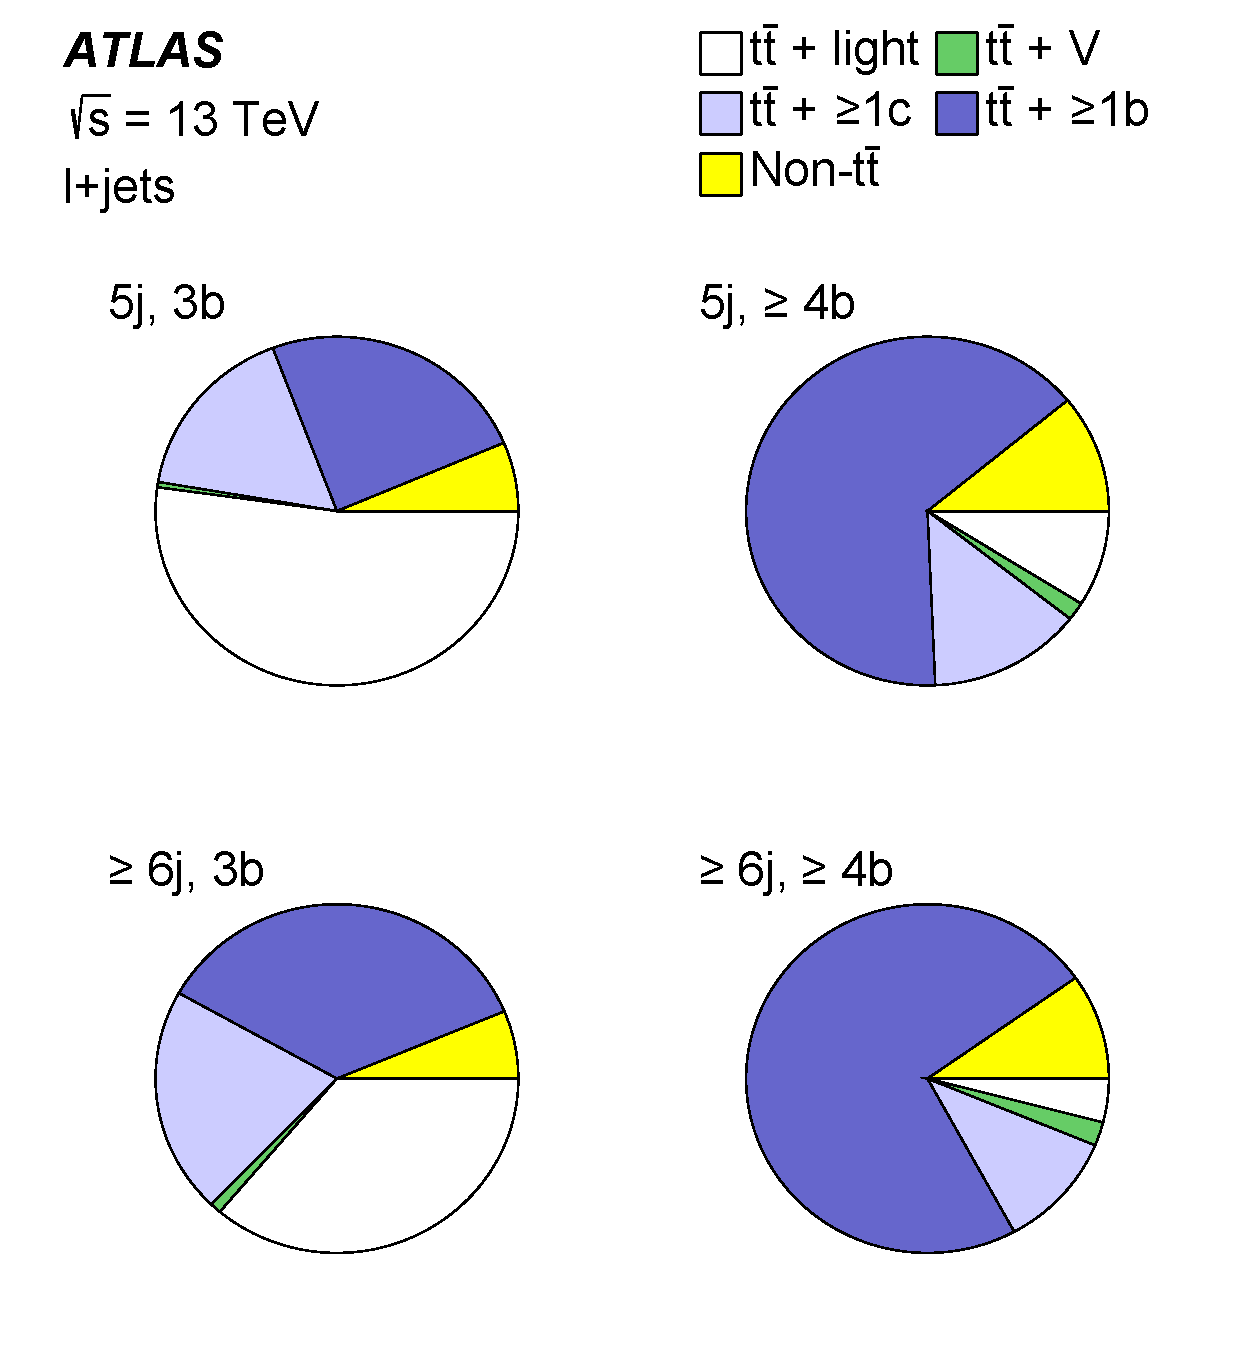
\includegraphics[width=0.75\textwidth]{TQX/cheeseplot.pdf}
    \caption{
        Background composition in the various analysis regions.
    }
    \label{tqX:cheeseplots}
    \end{center}
\end{figure}

Tables~\ref{tqX:prefityields2b1bl},~\ref{tqX:prefityields3b} and~\ref{tqX:prefityields4b} shows the number of expected and selected events in the different regions. The number of expected $t\to uX$ and $t\to cX$ signal events for the 60~GeV mass hypothesis is also shown, assuming a branching fraction B($t\to qX$)=0.1\%.\\

Figure~\ref{tqX:signalyields} shows the different signal yields and $\text{S}/\sqrt{\text{B}}$ for different analysis regions. The sensitivity for the 3b regions is larger than for the $\geq$4b, and increases with $m_{X}$ up to 140~GeV. The 20~GeV mass has significantly fewer yields, as the jets from the $X\to\bbar$ decay are mostly merged, thus often not selected. In addition, yields and sensitivity are higher for $t\to cX$ than for $t\to uX$, especially in the $\geq$4b regions, as expected.\\

Figure~\ref{tqX:acceptance} shows the acceptance times efficiency of the [4-6]j$\geq$3b inclusive selection per signal mass sample and for $t\to uX$ and $t\to cuX$, ranging from 0.2\% to 1.7\%. The acceptance and jet selection efficiency increase with the scalar mass as a consequence of the phase space dependence on the mass: the jets of the $b$-quark pair of the $X\to \bbar$ decay become merged at low $m_X$ because of the $X$ boost, reducing the jet multiplicity, while for high masses the jet from the $q$ is lost because of its smaller \pT.\\

\begin{table}[htb]
    \small
    \addtolength{\leftskip} {-4cm} % menja marges
    \addtolength{\rightskip}{-4cm}
    \centering
    \begin{tabular}{l r r r r r}
        \toprule\toprule
          & {4j, 2b+1bl} & {5j, 2b+1bl} & {6j, 2b+1bl} \\
          \midrule 
          $t\bar{t}$ + light        &  26100 $\pm$ 2700 & 17900 $\pm$ 2000 & 8000 $\pm$ 1800 \\ 
          $t\bar{t}$ + $\geq$1$b$   &  4600 $\pm$ 2500 & 6800 $\pm$ 3500 & 5400 $\pm$ 2800 \\ 
          $t\bar{t}$ + $\geq$1$c$   &  4900 $\pm$ 2500 & 6000 $\pm$ 3100 & 4200 $\pm$ 2200 \\ 
          $W\rightarrow cb$         &  210 $\pm$ 110 & 150 $\pm$ 80 & 70 $\pm$ 40   \\ 
          Single-top                &  1700  $\pm$ 500  & 1200  $\pm$ 400  & 620  $\pm$ 270  \\
          $t\bar{t}$ + $V$          &  90 $\pm$ 60 & 160 $\pm$ 100 & 160 $\pm$ 100    \\ 
          $VV$ \& $V$ + jets        &  870   $\pm$ 350  & 620   $\pm$ 70   & 350  $\pm$ 50   \\ 
          $t\bar{t}H+tH$            &  53    $\pm$ 6    & 133   $\pm$ 16    & 153  $\pm$ 18    \\         
\midrule      
Total                     & 38000 $\pm$ 5000 & 33000 $\pm$ 5000 & 19000 $\pm$ 4000  \\
\midrule
Data                      & 40889 & 35995 & 21210          \\

\midrule  
$t\to uX$ $m_X$=60 GeV             &  380 $\pm$ 40 & 293 $\pm$ 25 & 154 $\pm$ 32   \\
$t\to cX$ $m_X$=60 GeV             &  540 $\pm$ 50 & 372 $\pm$ 31 & 192 $\pm$ 35  \\
\bottomrule\bottomrule                               
    \end{tabular}
    \caption{Number of expected and selected events split according to the regions used to extract the reweighting factors for the \ttbar\ background and the signal, namely 4j2b+1bl, 5j2b+1bl and 6j2b+1bl. The quoted uncertainties include statistical and systematic uncertainties. The predicted number of $t\to uX$ and $t\to cX$ signal events for the 60~GeV mass hypothesis, assuming a branching fraction of 0.1\%, are also shown.
    }
    \label{tqX:prefityields2b1bl}
\end{table}

\begin{table}[htb]
    \small
    \addtolength{\leftskip} {-4cm} % menja marges
    \addtolength{\rightskip}{-4cm}
    \centering
    \begin{tabular}{l r r r r r}
        \toprule\toprule
        & {4j, 3b} & {5j, 3b} & {6j, 3b} \\
        \midrule 
        $t\bar{t}$ + light        &  11100 $\pm$ 1600  & 7800  $\pm$ 1500  & 3600  $\pm$ 900  \\ 
        $t\bar{t}$ + $\geq$1$b$   &  9000  $\pm$ 5000  & 14000 $\pm$ 7000  & 12000 $\pm$ 6000 \\ 
        $t\bar{t}$ + $\geq$1$c$   &  2500  $\pm$ 1300  & 3300  $\pm$ 1700  & 2400  $\pm$ 1300 \\ 
        $W\rightarrow cb$         &  380   $\pm$ 60    & 290   $\pm$ 50    & 143   $\pm$ 27   \\ 
        Single-top                &  1100  $\pm$ 400   & 1000  $\pm$ 400   & 570   $\pm$ 260  \\ 
        $t\bar{t}$ + $V$          &  130   $\pm$ 80    & 200   $\pm$ 120   & 210   $\pm$ 130  \\ 
        $VV$ \& $V$ + jets        &  690   $\pm$ 270   & 590   $\pm$ 50    & 350   $\pm$ 40   \\ 
        $t\bar{t}H+tH$            &  99    $\pm$ 15    & 266   $\pm$ 33    & 310   $\pm$ 40   \\              
\midrule      
Total                     &  25000 $\pm$ 4000  & 27000 $\pm$ 6000  & 19000 $\pm$ 5000 \\
\midrule
Data                      & 26614             & 28394          & 19302          \\
\midrule  
$t\to uX$ $m_X$=60 GeV             &  860 $\pm$ 90      & 690 $\pm$ 60    & 350 $\pm$ 40     \\
$t\to cX$ $m_X$=60 GeV             &  880 $\pm$ 90      & 690 $\pm$ 70    & 350 $\pm$ 40     \\
\bottomrule\bottomrule                               
    \end{tabular}
    \caption{
    Number of expected and selected events after applying reweighting split according to the signal regions,
namely 4j3b, 5j3b and 6j3b. The quoted uncertainties include both statistical and systematic uncertainties. The
predicted number of $t\to uX$ and $t\to cX$ signal events for the 60 GeV mass hypothesis, assuming a branching
fraction of 0.1\%, are also shown.
    }
    \label{tqX:prefityields3b}
\end{table}

\begin{table}[htb]
    \small
    \addtolength{\leftskip} {-4cm} % menja marges
    \addtolength{\rightskip}{-4cm}
    \centering
    \begin{tabular}{l r r r r r}
        \toprule\toprule
        & {4j, 4b} & {5j, $\ge$4b} & {6j, $\ge$4b} \\
        \midrule 
        $t\bar{t}$ + light        &  5.1 $\pm$ 3.5 & 8   $\pm$ 6   & 6    $\pm$ 6   \\ 
        $t\bar{t}$ + $\geq$1$b$   &  250 $\pm$ 140 & 900 $\pm$ 500 & 1200 $\pm$ 700 \\ 
        $t\bar{t}$ + $\geq$1$c$   &  10  $\pm$ 7   & 26  $\pm$ 14  & 25   $\pm$ 14  \\ 
        $W\rightarrow cb$         & 8.3 $\pm$ 1.3 & 11.9 $\pm$ 2.1   & 8.3 $\pm$ 2.8     \\ 
        Single-top                & 22  $\pm$ 14  & 42   $\pm$ 19    & 50 $\pm$ 32 \\ 
        $t\bar{t}$ + $V$          & 7 $\pm$ 5  & 26 $\pm$ 16  & 36 $\pm$ 22     \\ 
        $VV$ \& $V$ + jets        &  13 $\pm$ 5  & 22.7 $\pm$ 3.0  & 20.2 $\pm$ 2.7    \\ 
        $t\bar{t}H$               & 6.2 $\pm$ 1.1 &  44 $\pm$ 7  & 76 $\pm$ 11   \\                   
\midrule      
Total                     & 320 $\pm$ 140  & 1100 $\pm$ 500  & 1500 $\pm$ 700  \\
\midrule
Data                      & 374               & 1179          & 1492          \\
\midrule  
$t\to uX$ $m_X$=60 GeV             &  2.8 $\pm$ 1.3      & 8.6 $\pm$ 3    &  14 $\pm$ 7     \\
$t\to cX$ $m_X$=60 GeV             &  17  $\pm$ 6        & 27  $\pm$ 8    & 24 $\pm$ 12     \\
\bottomrule\bottomrule                               
    \end{tabular}
    \caption{
Number of expected and selected events after applying reweighting split according to the control regions,
namely 4j4b, 5j$\geq$4b and 6j$\geq$4b. The quoted uncertainties include both statistical and systematic uncertainties. The predicted number of $t\to uX$ and $t\to cX$ signal events for the 60 GeV mass hypothesis, assuming a branching
fraction of 0.1\%, are also shown.
    }
    \label{tqX:prefityields4b}
\end{table}

\begin{figure}[htbp]
    \RawFloats
    \begin{center}
        \subfloat[2b1bl regions yields]{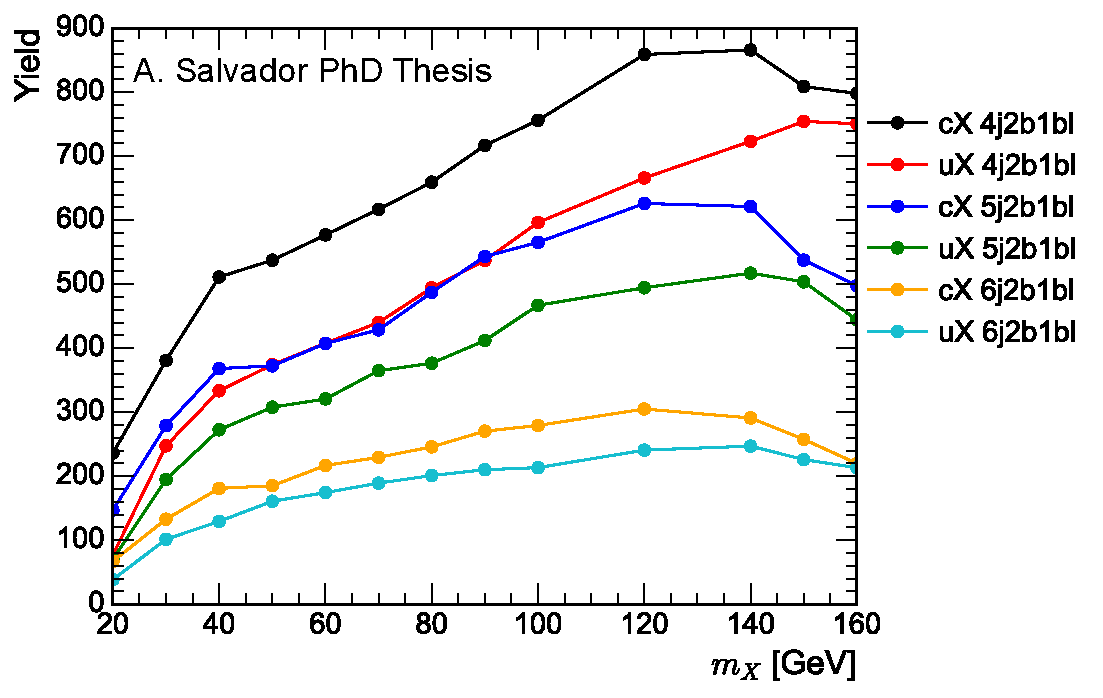
\includegraphics[width = 0.5\textwidth]{TQX/Yieldplot_2b.pdf}}
        \subfloat[2b1bl regions $\text{S}/\sqrt{\text{B}}$]{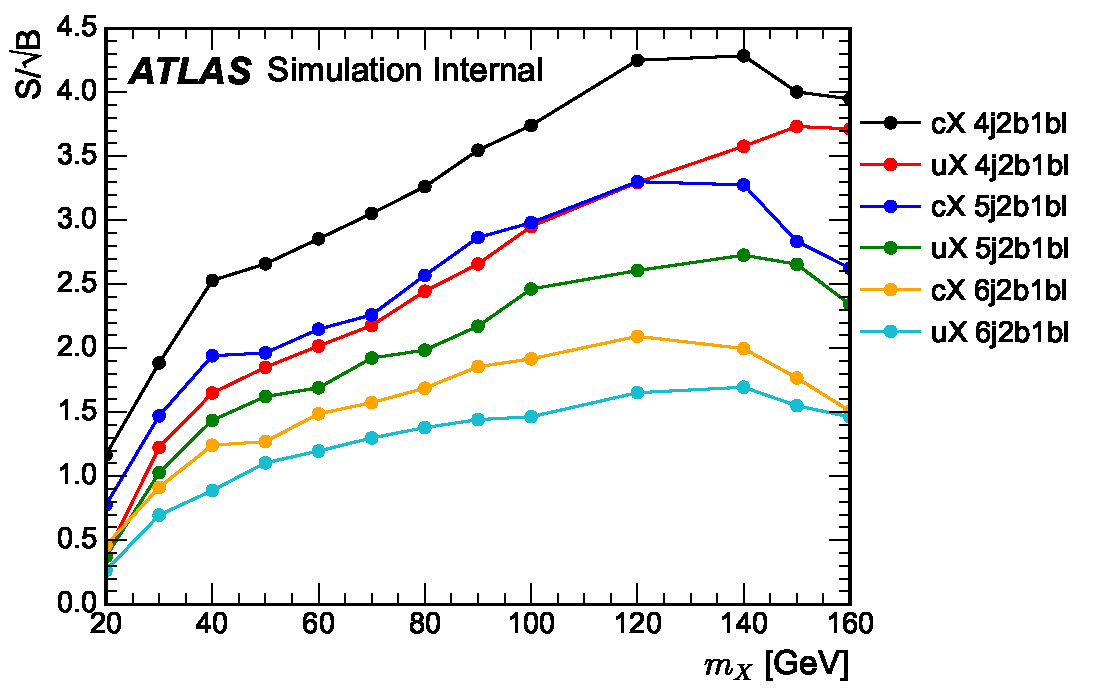
\includegraphics[width = 0.5\textwidth]{TQX/SsqrtBplot_2b.pdf}} \\
        \subfloat[3b regions yields]{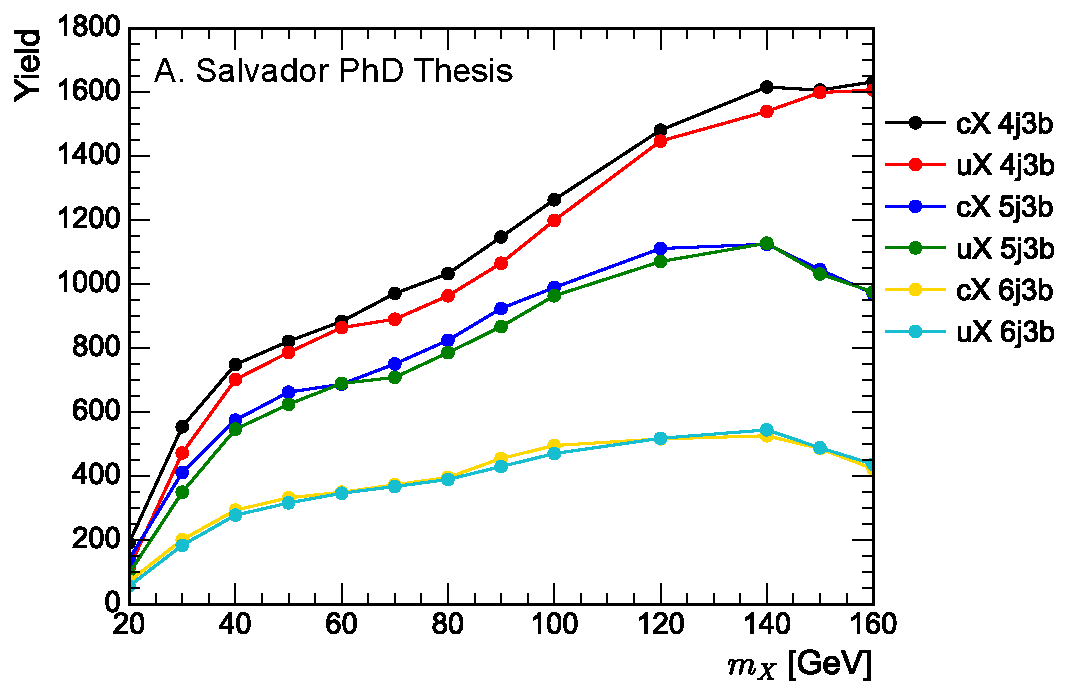
\includegraphics[width = 0.5\textwidth]{TQX/Yieldplot_3b.pdf}}
        \subfloat[3b regions $\text{S}/\sqrt{\text{B}}$]{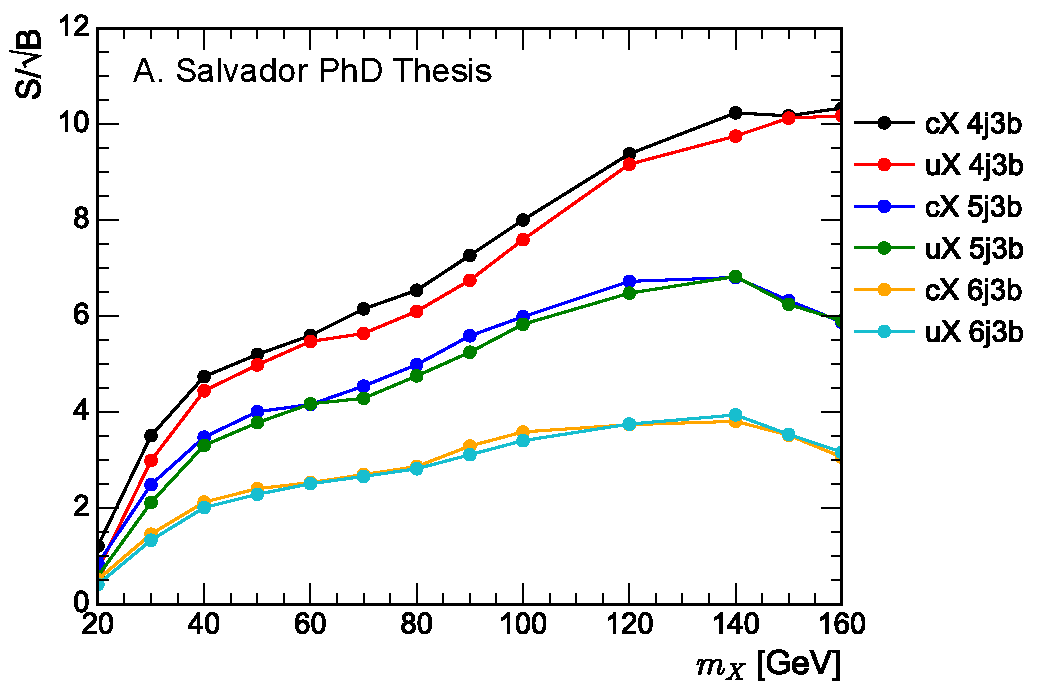
\includegraphics[width = 0.5\textwidth]{TQX/SsqrtBplot_3b.pdf}} \\
        \subfloat[$\geq$4b yields]{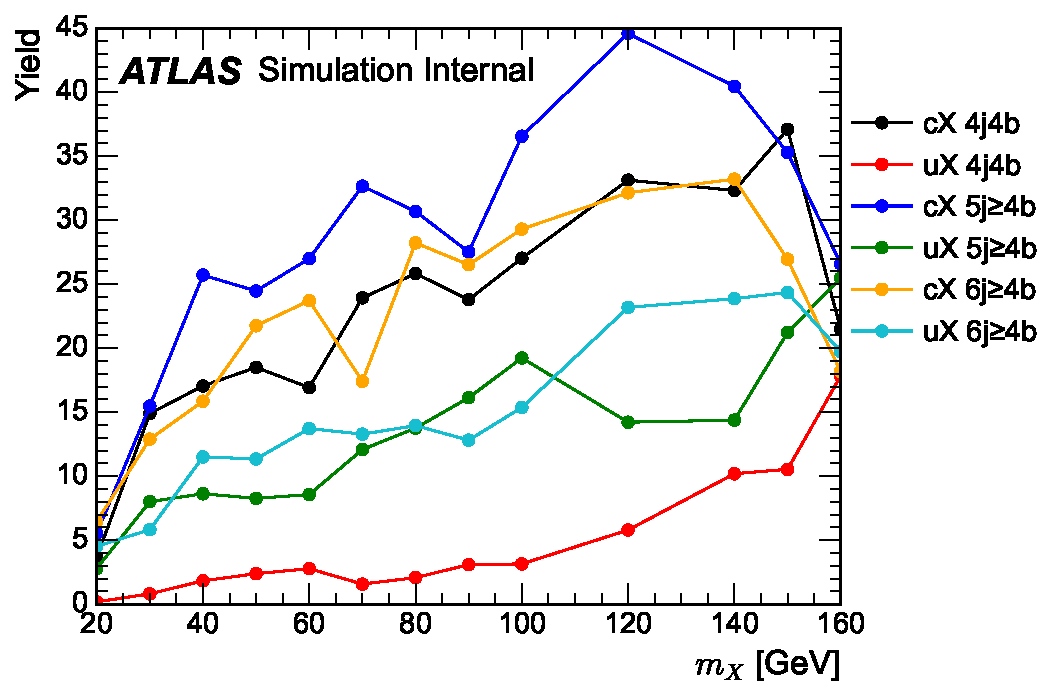
\includegraphics[width = 0.5\textwidth]{TQX/Yieldplot_4b.pdf}}
        \subfloat[$\geq$4b $\text{S}/\sqrt{\text{B}}$]{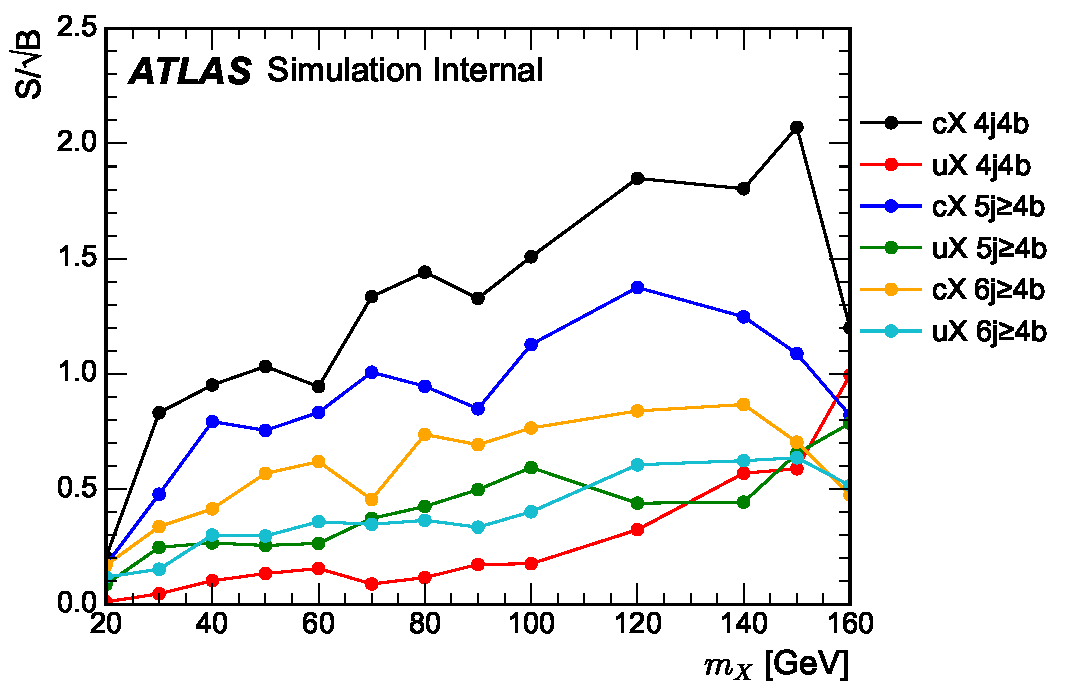
\includegraphics[width = 0.5\textwidth]{TQX/SsqrtBplot_4b.pdf}} \\
    \caption{
        Signal yields (left) and $\text{S}/\sqrt{\text{B}}$ (right) for the 2b+1bl (top), 3b (middle) and $\geq$4b (bottom) regions after applying reweighting as a function of the mass of $X$ for both $t\to qX$ processes, assuming a branching fraction of 0.1\% and an integrated luminosity of 139~fb$^{-1}$.
    }
    \label{tqX:signalyields}
    \end{center}
\end{figure}

\begin{figure}[htbp]
    \RawFloats
    \begin{center}
    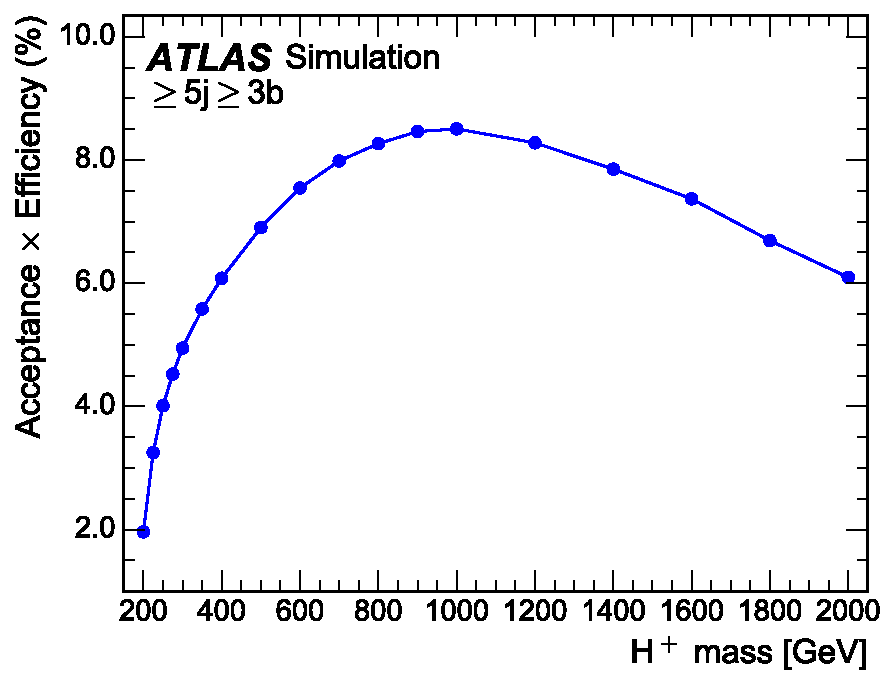
\includegraphics[width=0.75\textwidth]{TQX/acceptance.pdf}
    \caption{
        Acceptance times efficiency of the signal regions as a function of the scalar signal mass corresponding to
the $t\to uX$ and $t\to cX$ channels.
    }
    \label{tqX:acceptance}
    \end{center}
\end{figure}

\clearpage
\subsection{Reweighting technique}
\label{tqX:secRW}
The main background for the search is \ttjets, and its correct modelling is essential for the correct description of the data. As mentioned for the $H^\to tb$ analysis (Section~\ref{Hplustb:secRW}), the simulation does not properly model high jet multiplicities nor the hardness of additional jet emissions and data-based corrections are applied to improve the data/MC agreement.\\

The correction factors are applied to the \ttbar\ samples as well as the signal samples, as they are modelled as using the same \acrshort{MClabel} generator. The corrections derived in the 2b+1bl regions are expected to improve the agreement in the 3b and $\geq$4b regions. The remaining discrepancies can be covered by the systematic model.\\

The corrections are derived for each jet multiplicity and as a function of \HTall, defined as the scalar \pT sum of jets, the lepton and \MET. The reweighting factors for each jet multiplicity is expressed as:

\begin{equation}
    \label{tqX:RWeq}
    R(\HTall)=\frac{ \text{Data}(\HTall) - \text{MC}^{\text{non-\ttbar}(\HTall)} }{\text{MC}^{\text{\ttbar}(\HTall)}}
\end{equation}

and, by construction, assumes that any disagreement between data and MC comes from \ttbar.\\

Figure~\ref{tqX:RWfactors} includes all the derived corrections, showing higher weights for increased jet multiplicities and, in general, the \HTall\ corrections have a hyperbolic behaviour: close to one for $\HTall > 800$~GeV and rapidly increasing towards lower values of \HTall. Among various functions, the hyperbolic function was found to best fit the \HTall\ weight distributions: $w=A+\frac{B}{(\HTall)^C}$. The eigenvalues of the error matrix of fitted parameters are included as systematic uncertainties.\\

\begin{figure}[htb]
    \RawFloats
    \begin{center}
    \subfloat[4j2b+1bl]{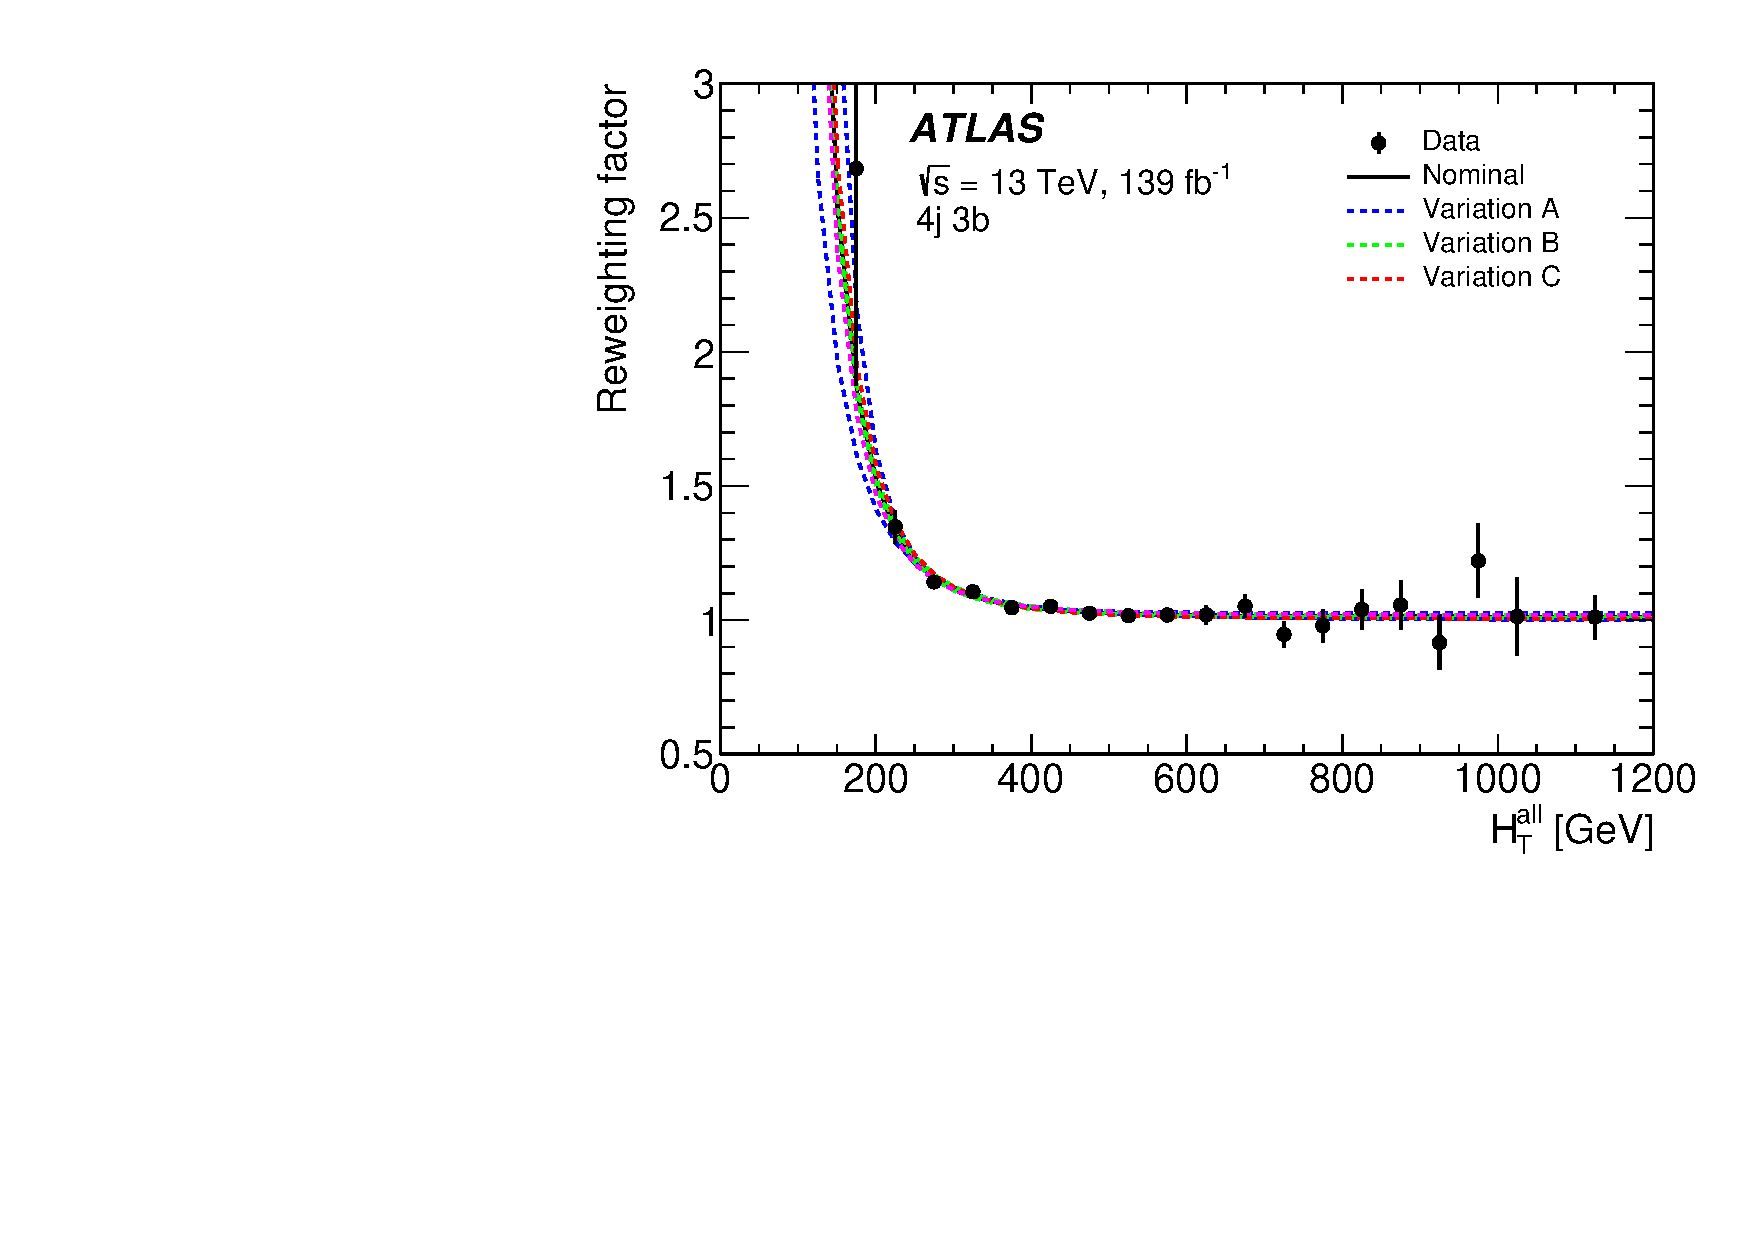
\includegraphics[width = 0.5\textwidth]{TQX/Reweighting/RWfigure_4j.pdf}} \\
    \subfloat[5j2b+1bl]{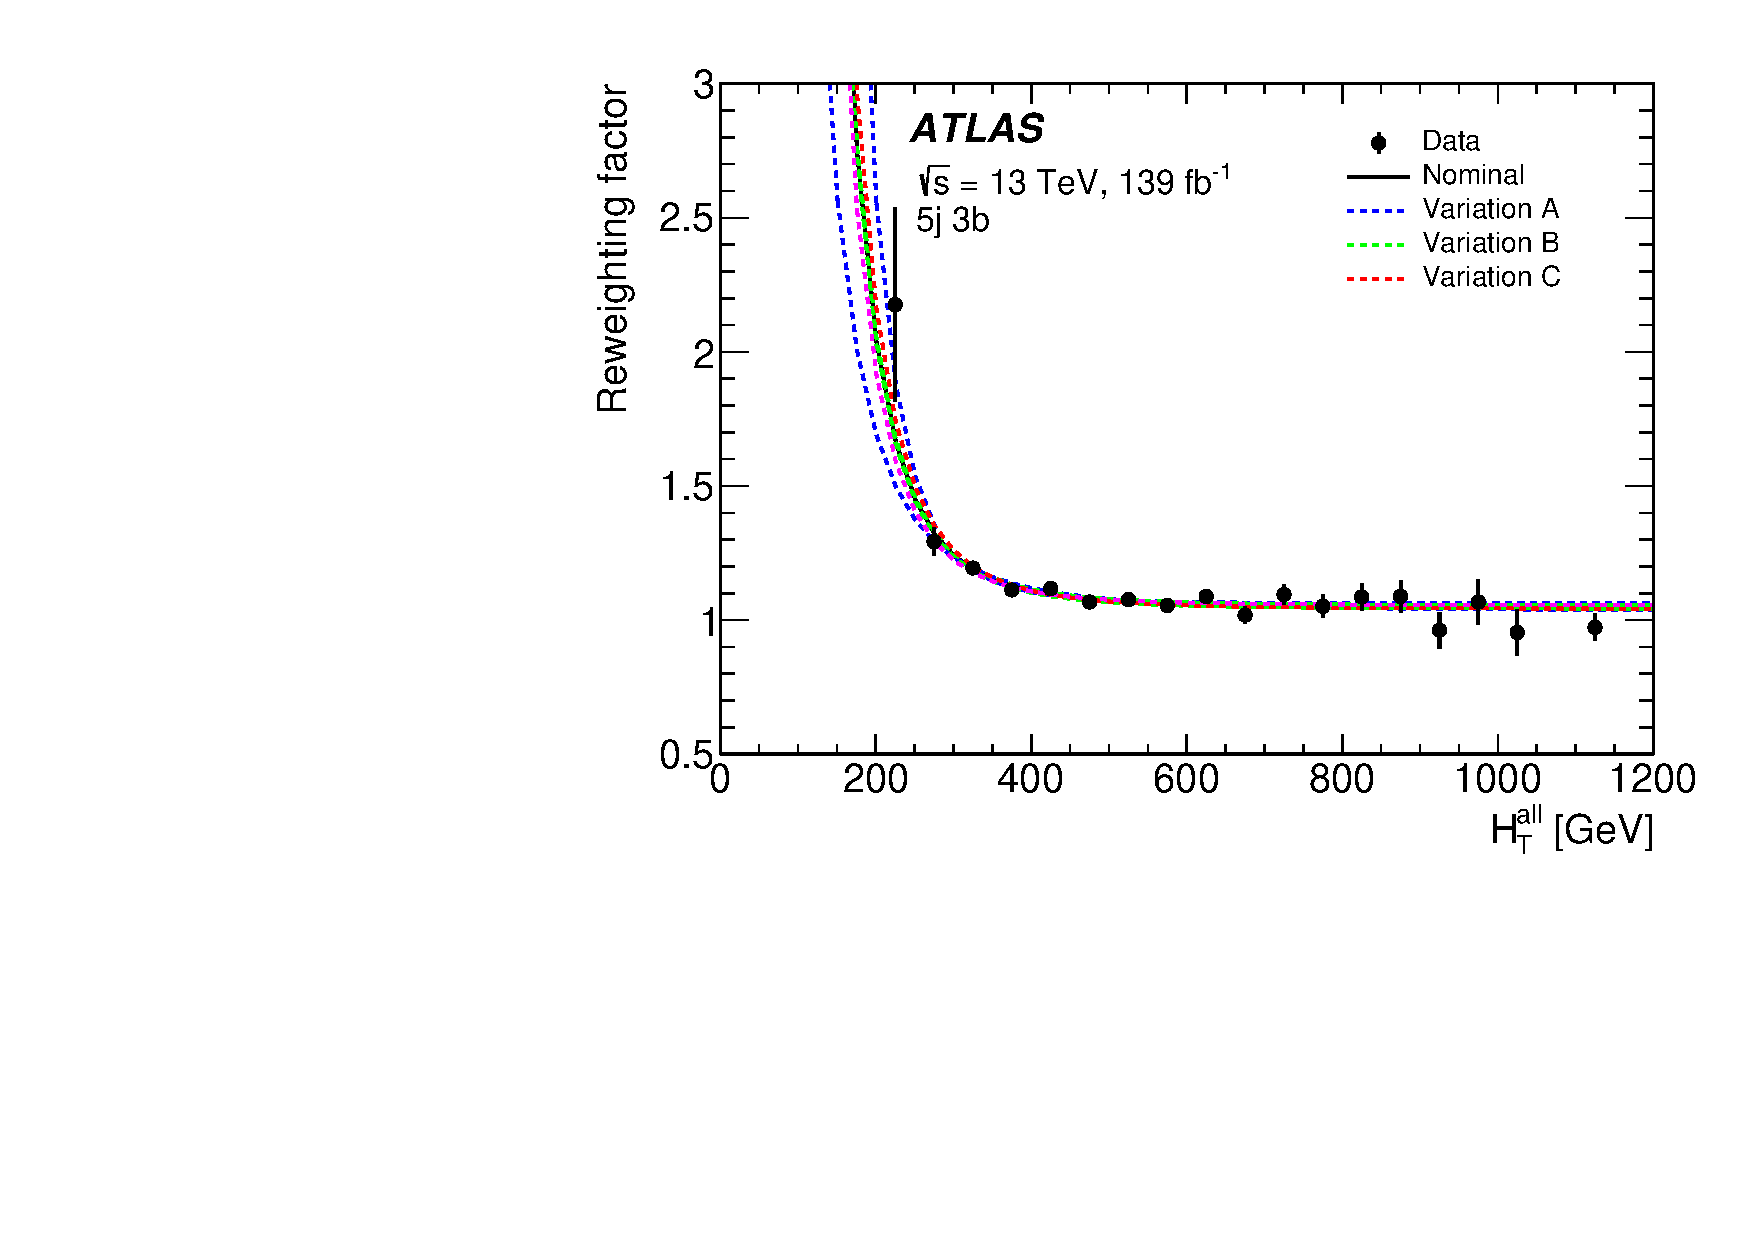
\includegraphics[width = 0.5\textwidth]{TQX/Reweighting/RWfigure_5j.pdf}} 
    \subfloat[6j2b+1bl]{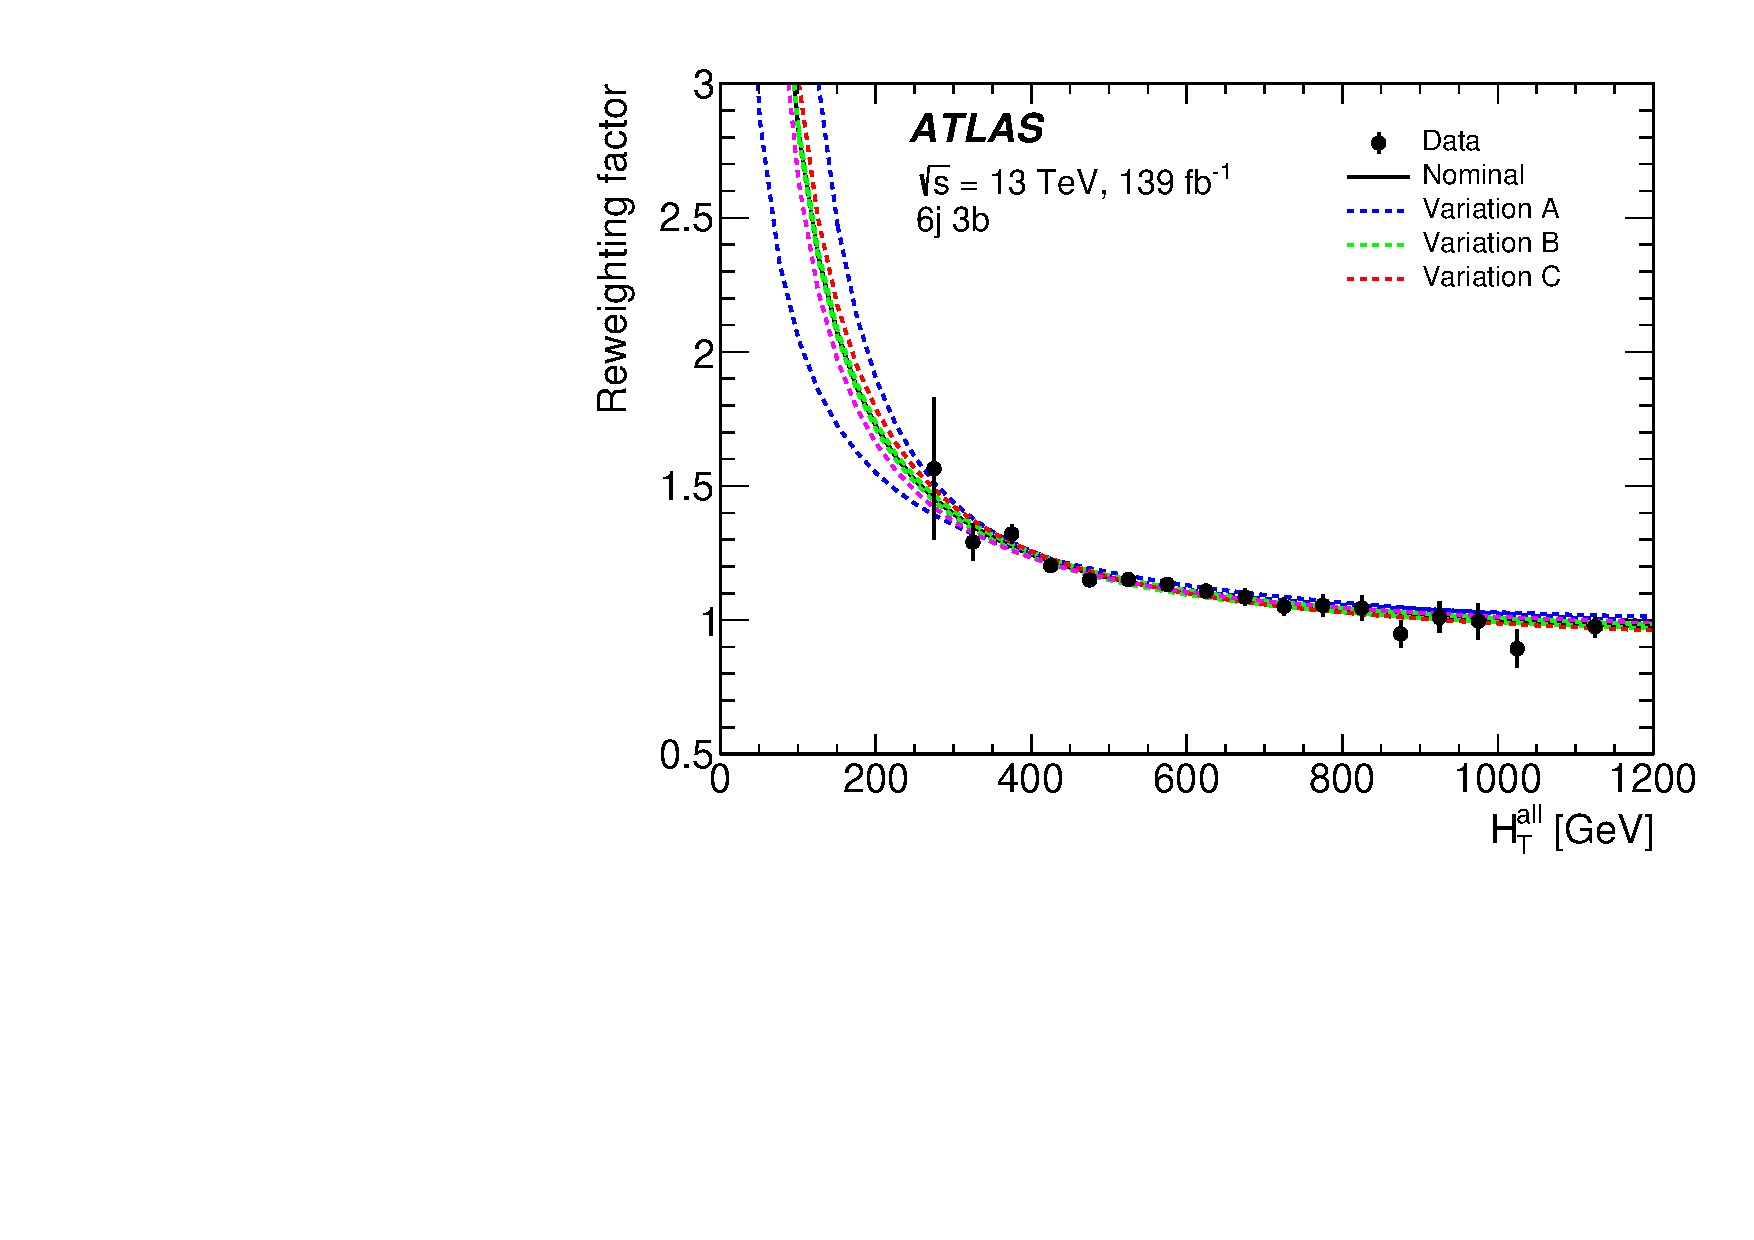
\includegraphics[width = 0.5\textwidth]{TQX/Reweighting/RWfigure_6j.pdf}}
    \caption{Reweighting factors (weights) obtained from the comparison between data and simulation of the number of \HTall\ for the 2b+1bl regions and three different jet multiplicities, with the uncertainty bands associated to the variations of the eigenvalues of the matrix error of the fit function, namely $A$, $B$ and $C$. The errors in the data points include the statistical uncertainties in data and \acrshort{MClabel} predictions.}
    \label{tqX:RWfactors}
\end{center}
\end{figure}

The agreement between simulation and data in the analysis region improves, as an example, Figure~\ref{tqX:RWeffect} shows the leading jet \pT\ distribution before and after the reweighting, which improves especially at low values. All studies included in this thesis are shown after the reweighting corrections are applied, unless stated otherwise.\\

\begin{figure}[htb]
    \RawFloats
    \begin{center}
    \subfloat[4j3b, unweighted]
    {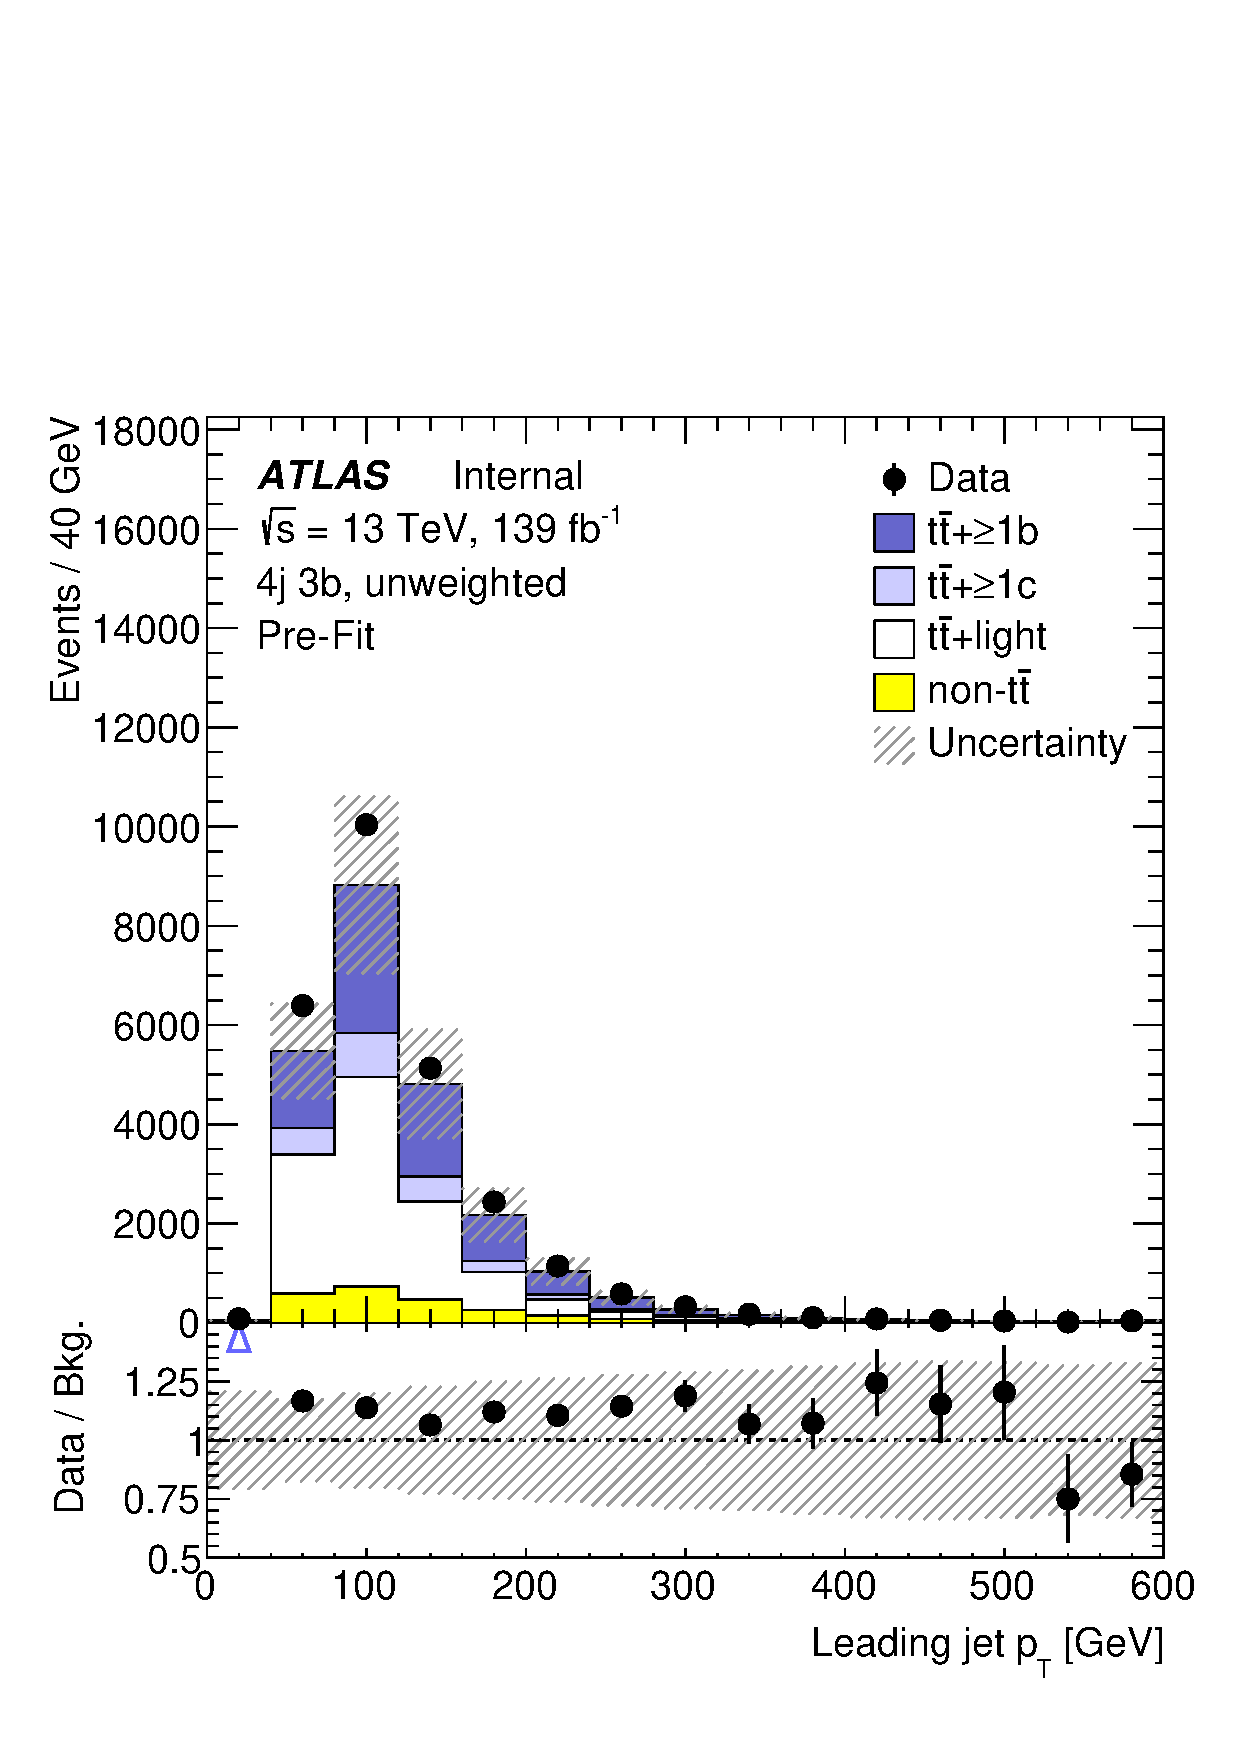
\includegraphics[width = 0.33\textwidth]{TQX/Reweighting/jet0_ptv2_4jex3bex_noRW.pdf}}
    \subfloat[4j3b, reweighted] 
    {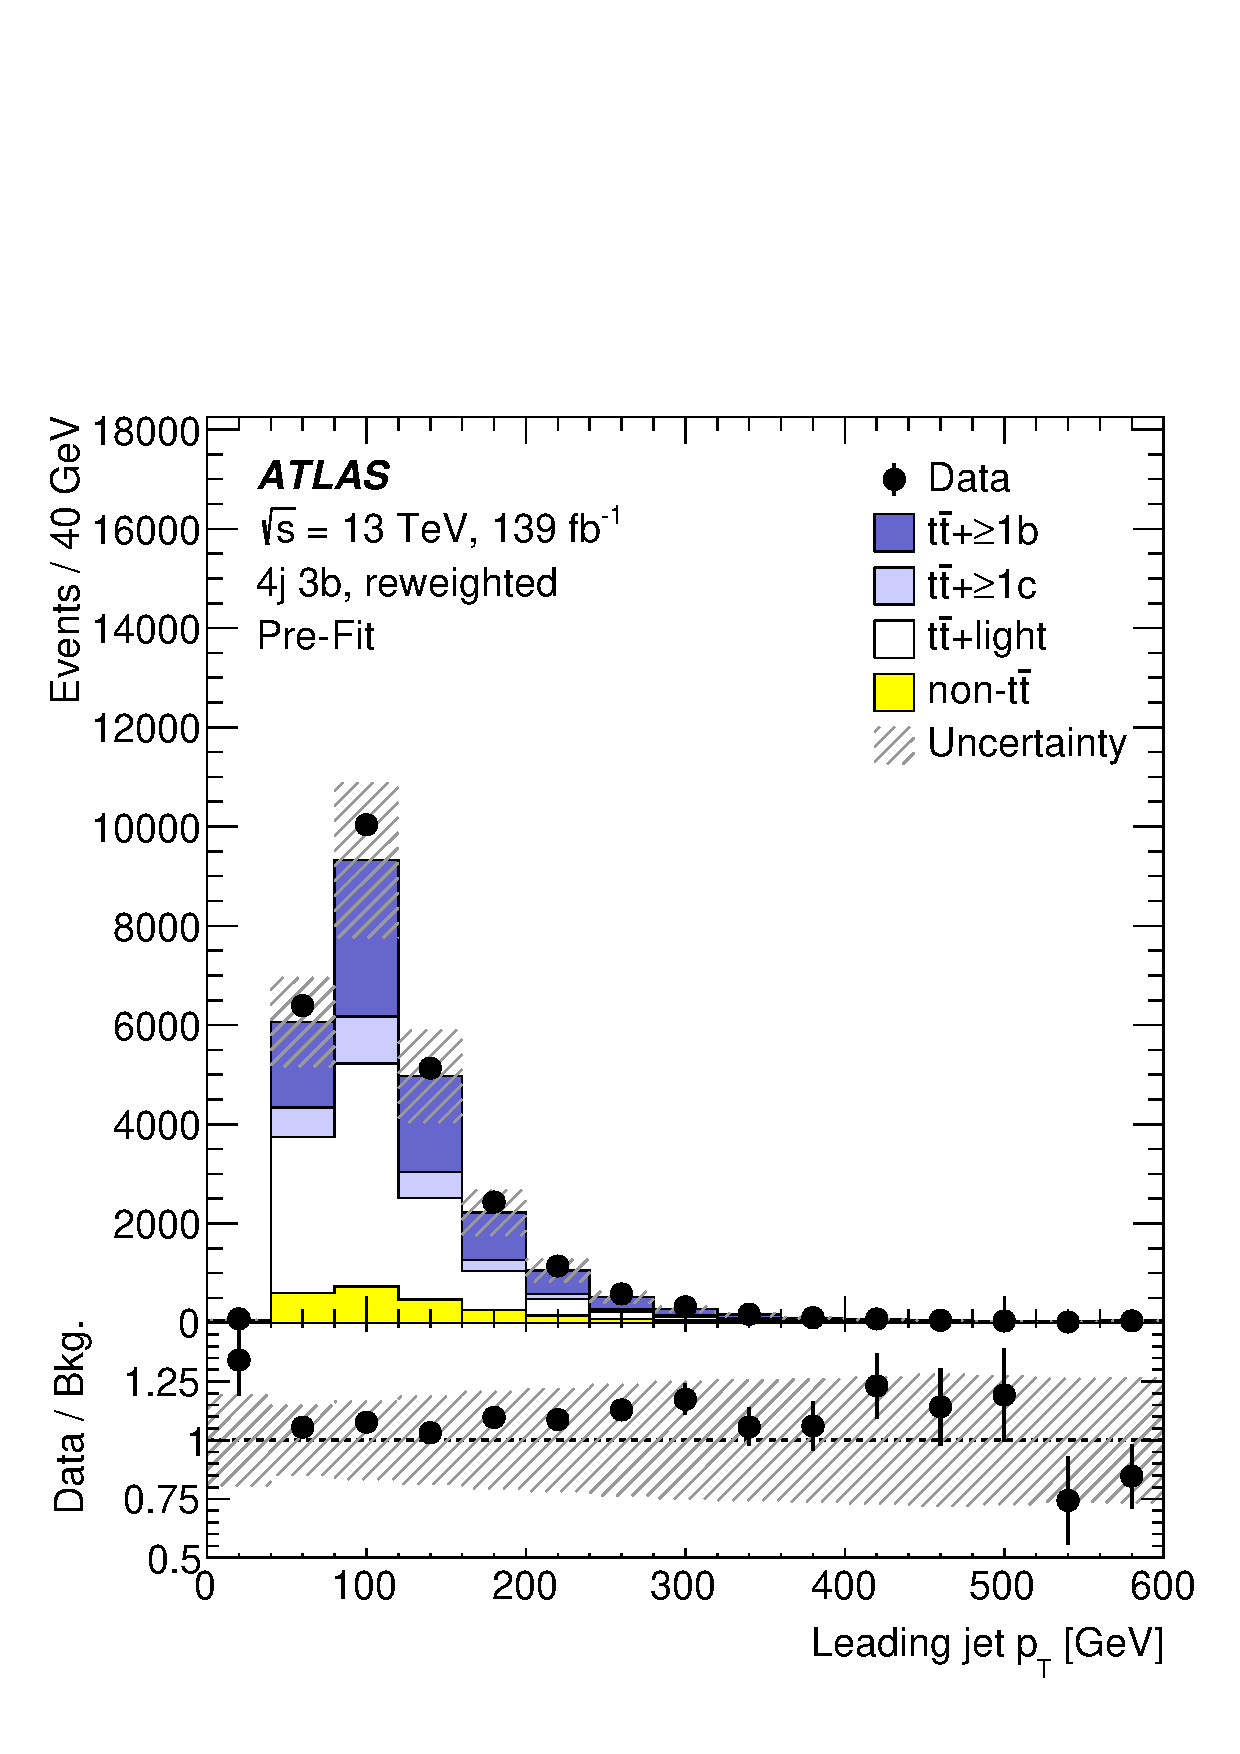
\includegraphics[width = 0.33\textwidth]{TQX/Reweighting/jet0_ptv2_4jex3bex.pdf}} \\
    \subfloat[5j3b, unweighted]
    {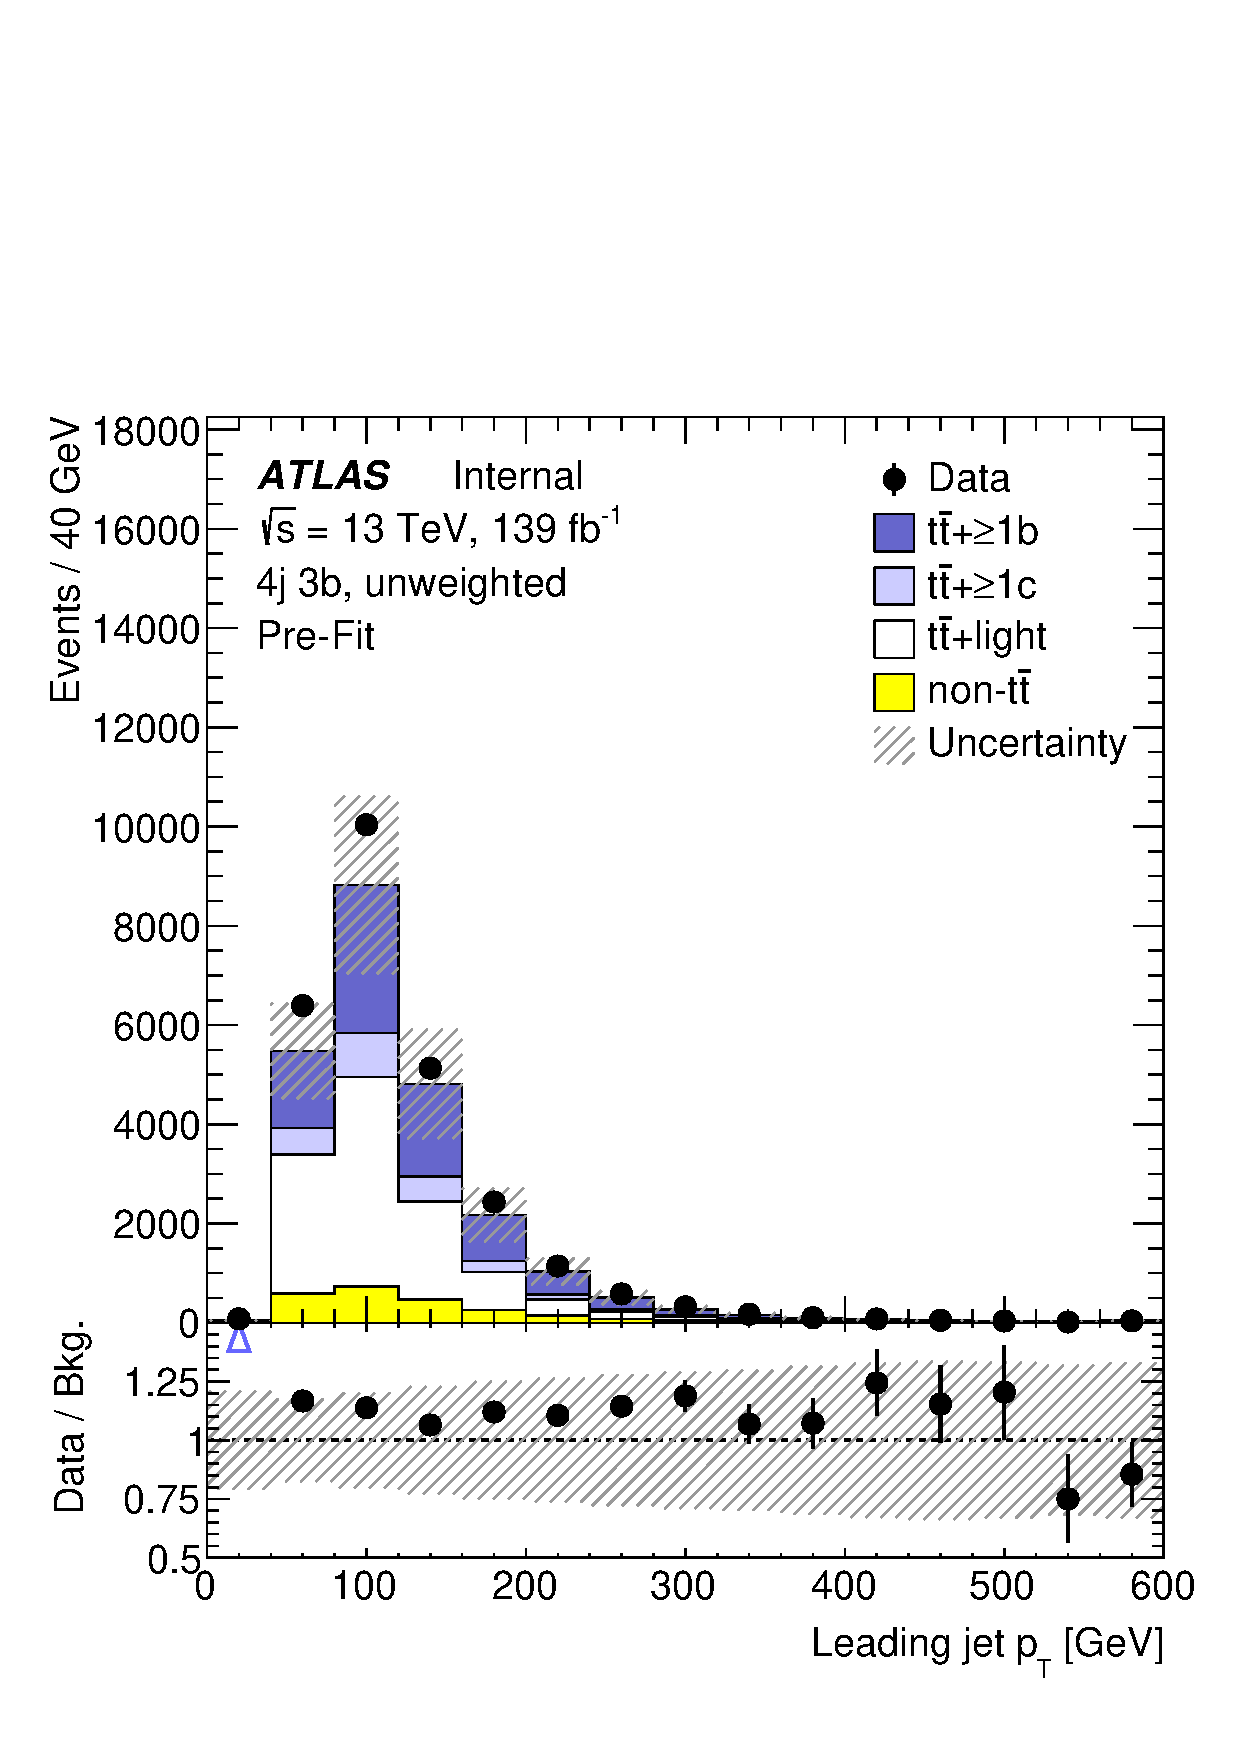
\includegraphics[width = 0.33\textwidth]{TQX/Reweighting/jet0_ptv2_4jex3bex_noRW.pdf}}
    \subfloat[5j3b, reweighted] 
    {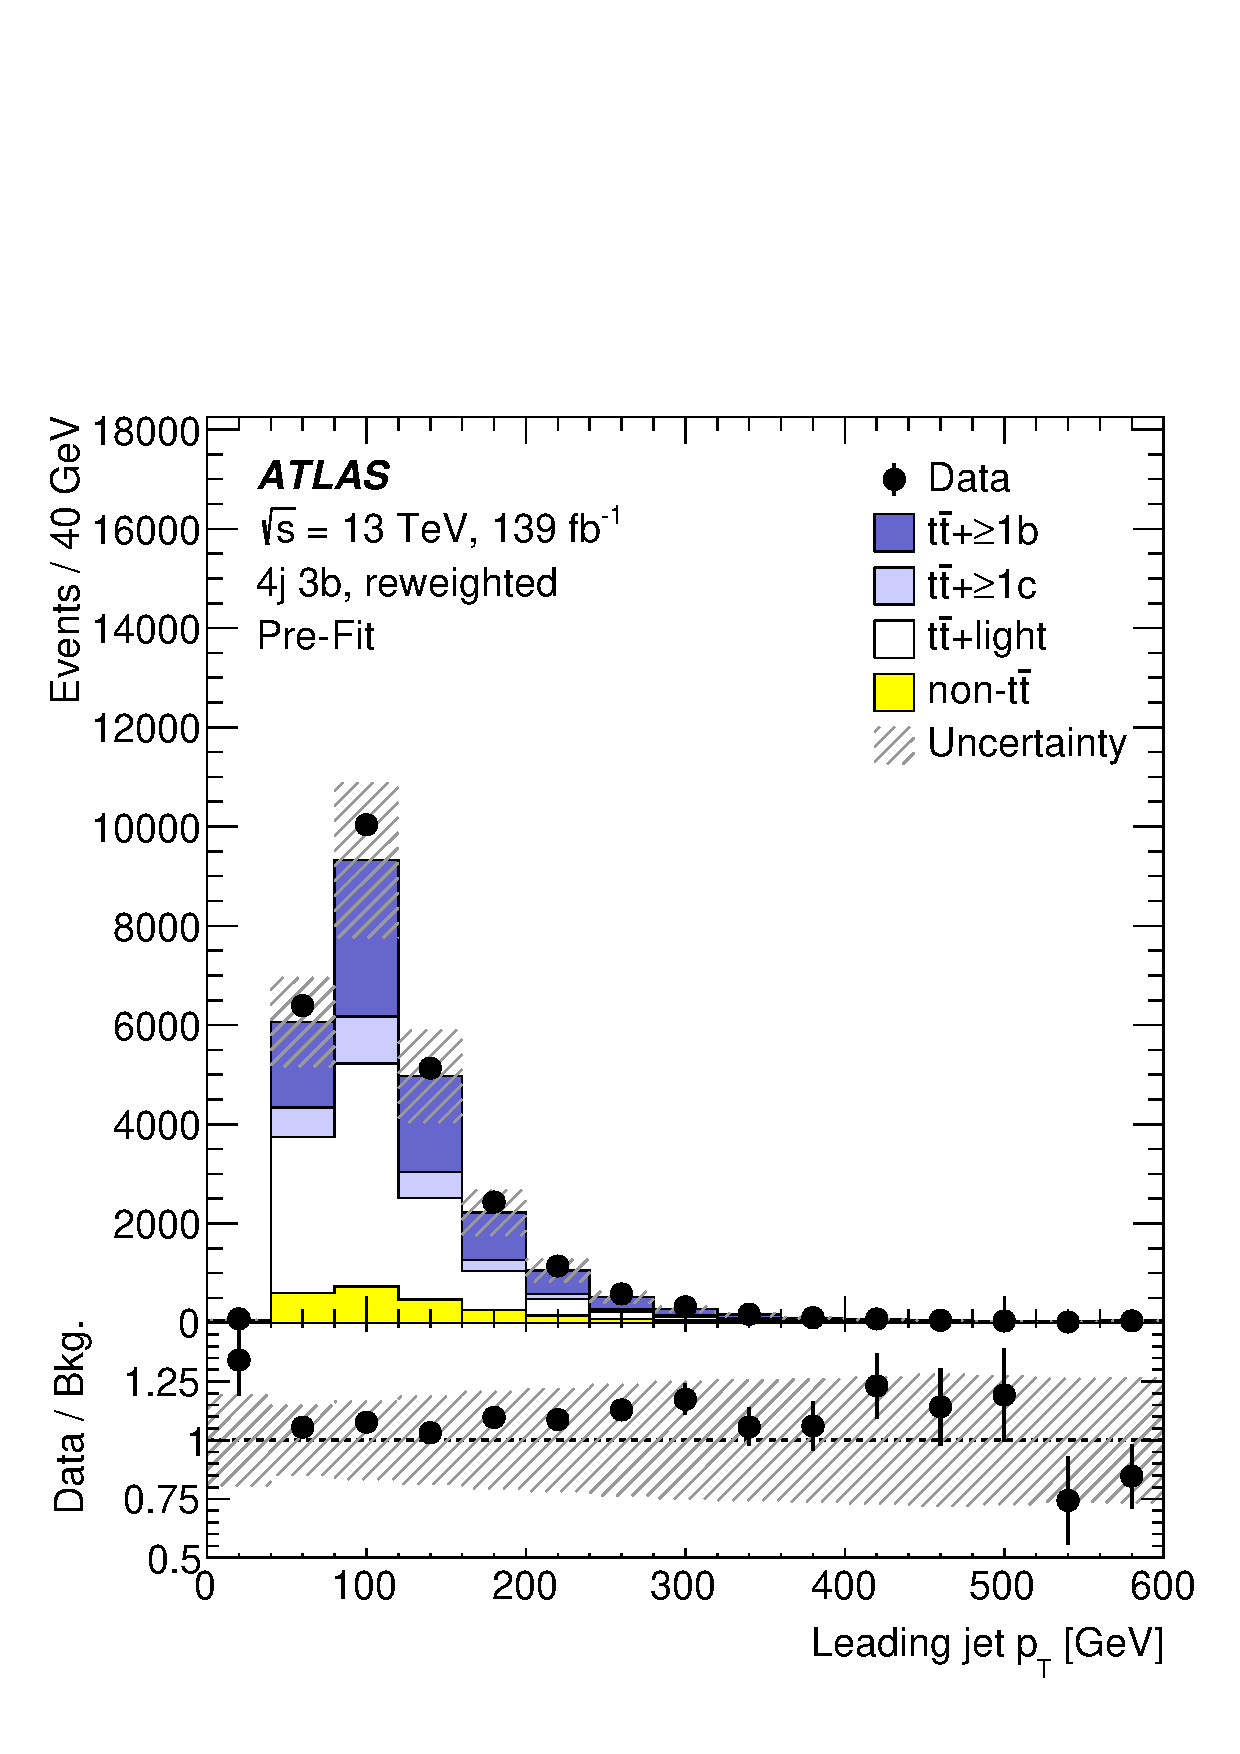
\includegraphics[width = 0.33\textwidth]{TQX/Reweighting/jet0_ptv2_4jex3bex.pdf}} \\
    \subfloat[6j3b, unweighted]
    {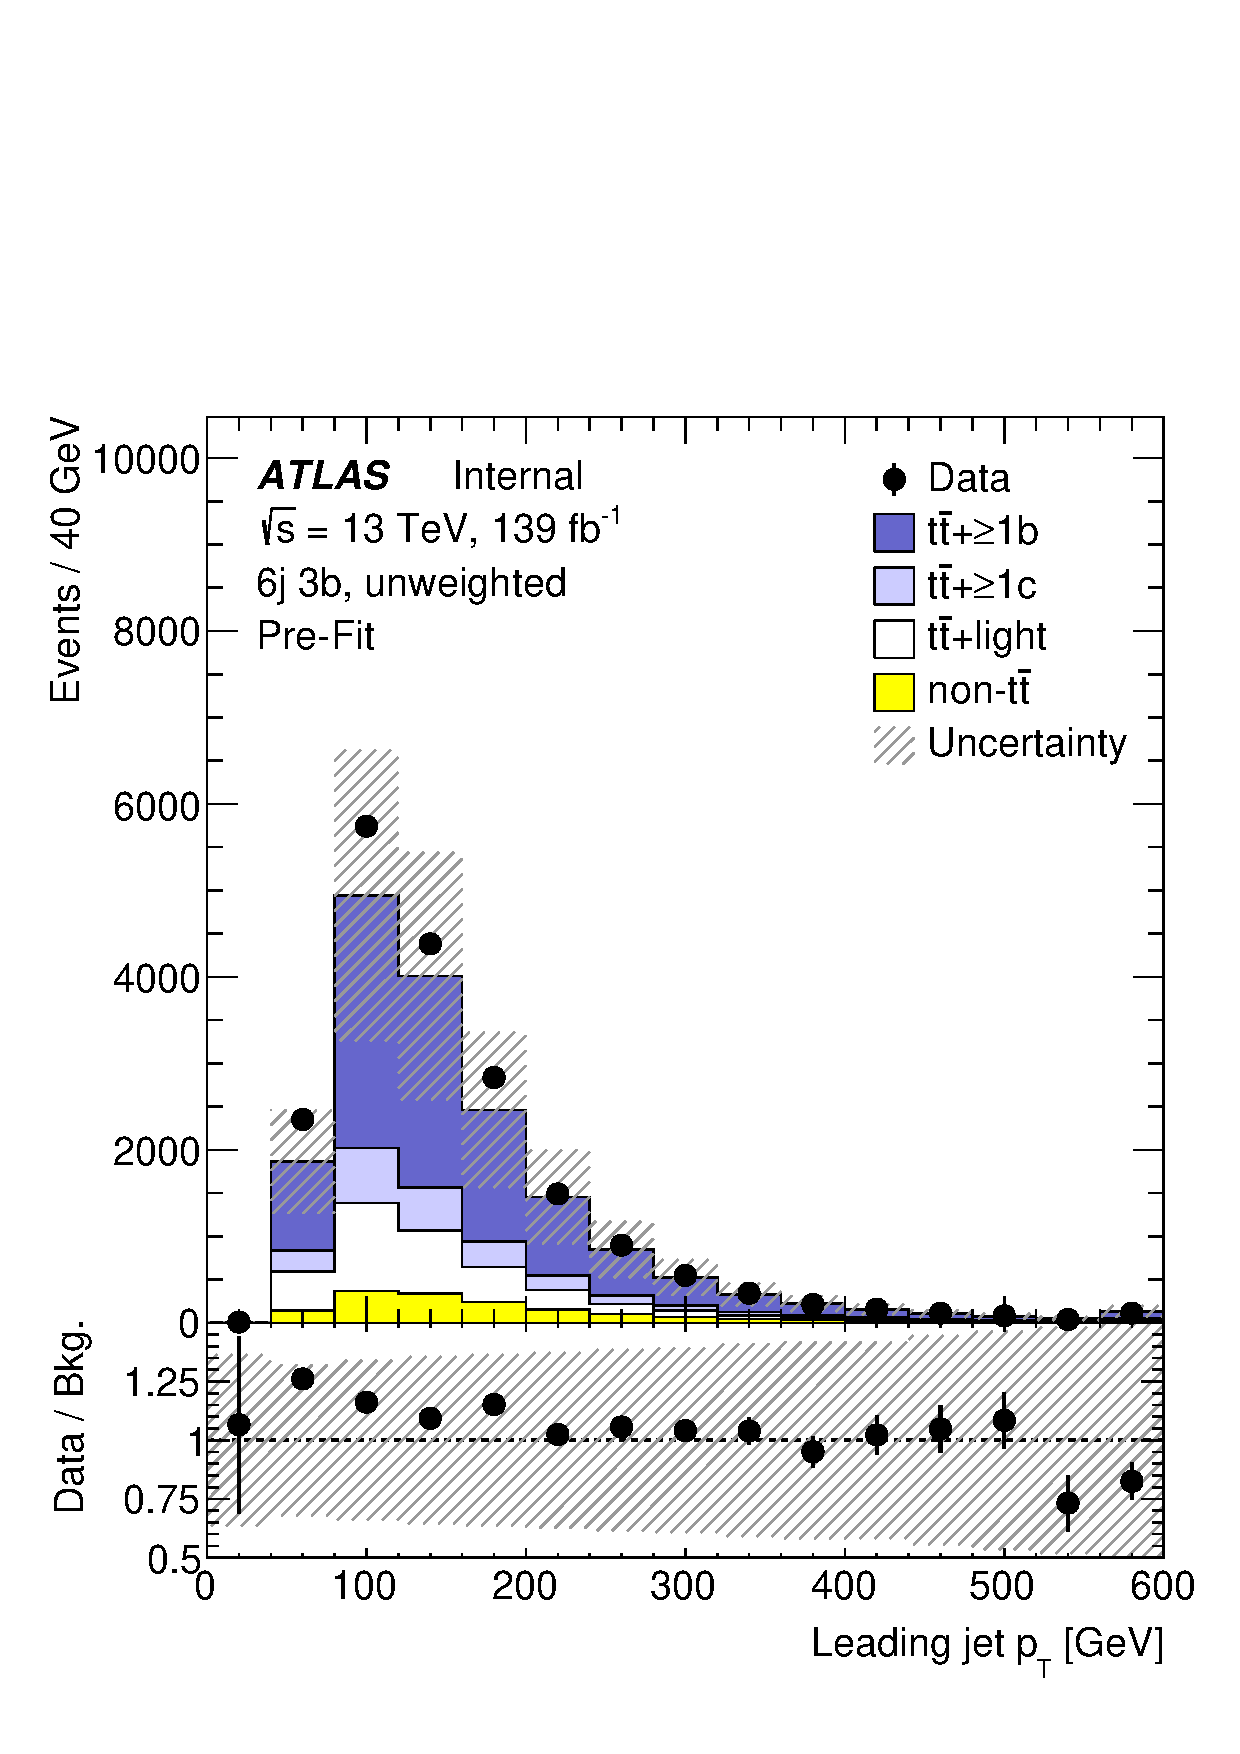
\includegraphics[width = 0.33\textwidth]{TQX/Reweighting/jet0_ptv2_6jex3bex_noRW.pdf}}
    \subfloat[6j3b, reweighted] 
    {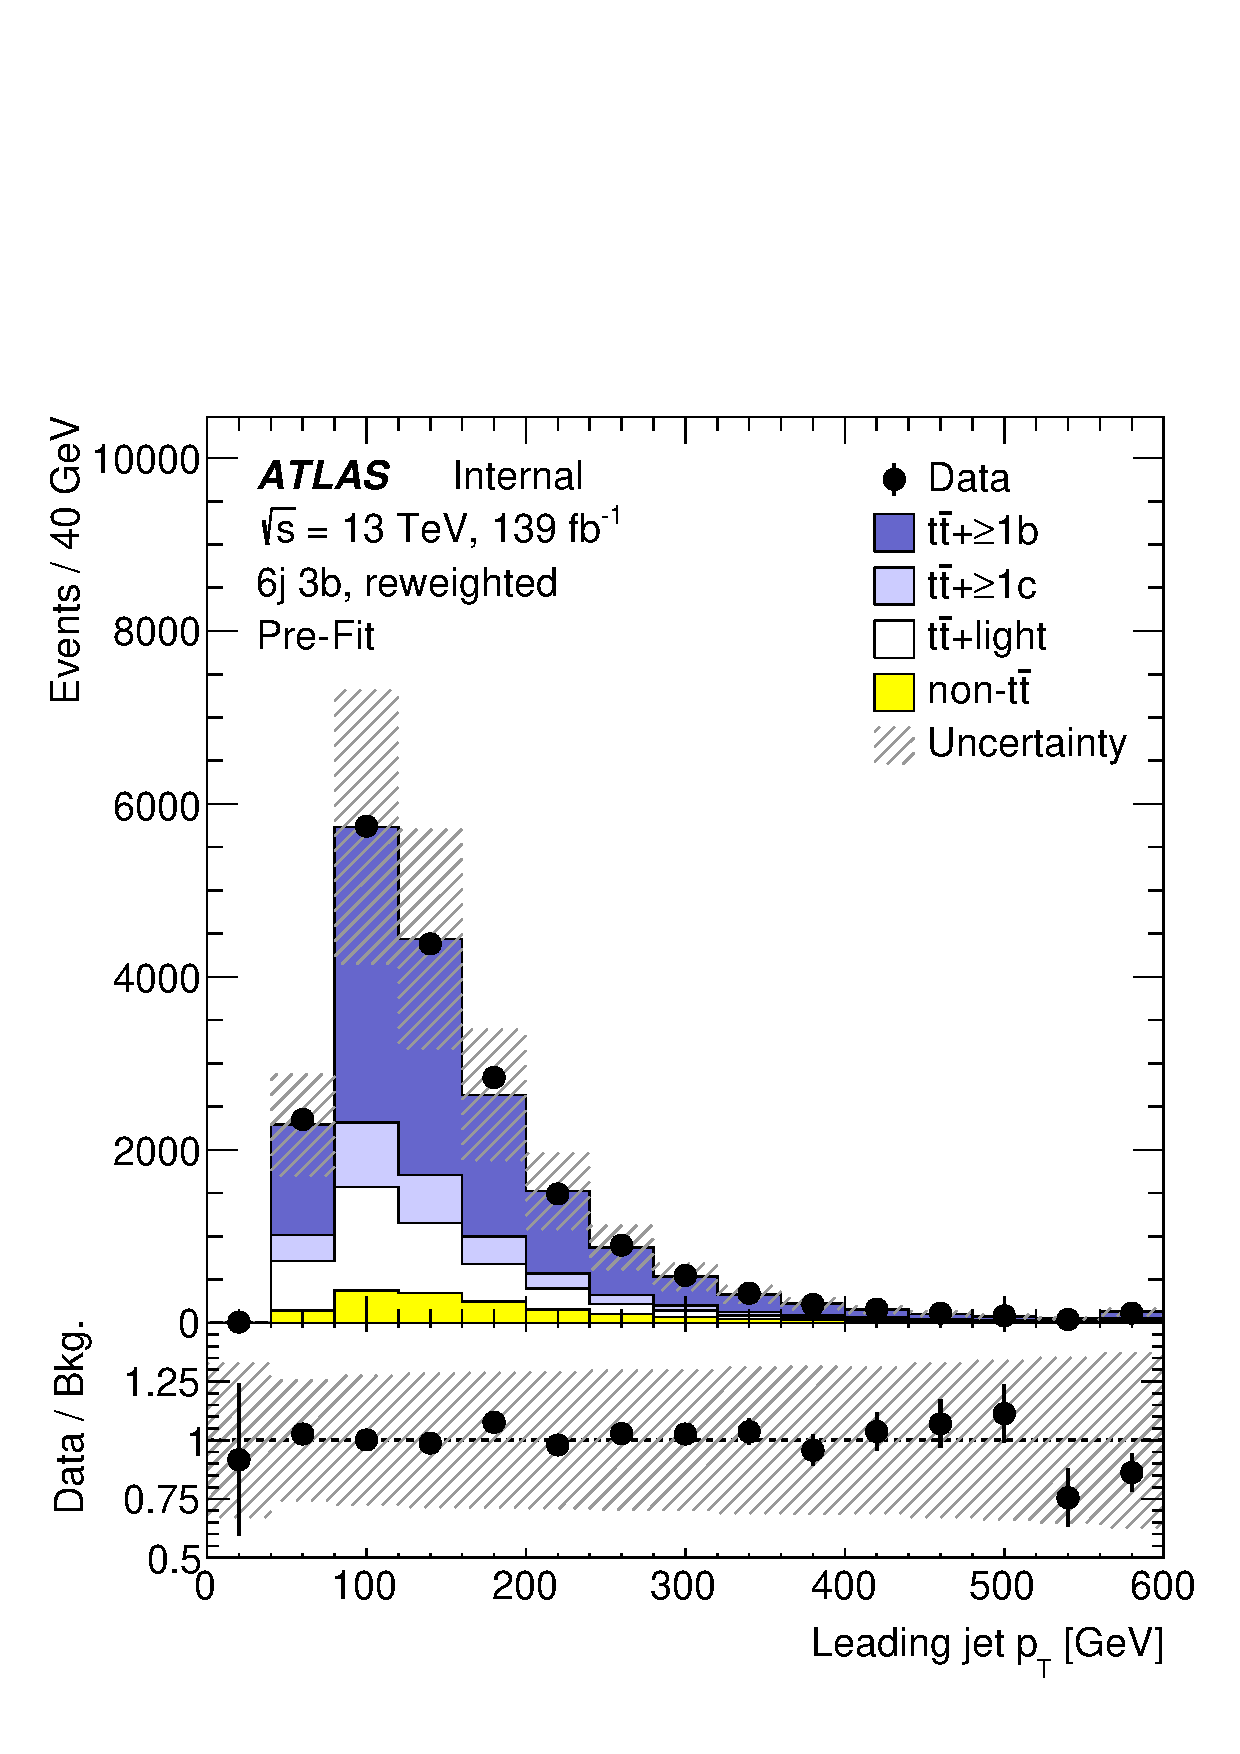
\includegraphics[width = 0.33\textwidth]{TQX/Reweighting/jet0_ptv2_6jex3bex.pdf}} \\
    \caption{
    Distributions of the leading jet \pT\ before the fit to the data in the different 3b analysis regions before (left) and after (right) applying the \HTall-based reweighting. The last bin includes the overflows. 
    The lower panels display the ratio of the data to the total prediction.
    The hatched bands show the uncertainties before the fit to the data and include the correlated systematic uncertainties in the prediction and the statistical uncertainties uncorrelated across bins. When the reweighting is applied, the uncertainty bands are computed accordingly and include the associated uncertainties.    
    }
    \label{tqX:RWeffect}
\end{center}
\end{figure}
\clearpage
\subsection{Multivariate techniques}

Multivariate techniques are used in this analysis to enhance the separation between signal and background. The kinematics of \ttb\ and signal events are very similar, and these methods can use different distributions as inputs to obtain a powerful discriminating variable.\\

The main classifier is a parameterised NN trained over all masses for each $t\to qX$ signal process and background, implemented with the same software tools as the $H^+\to tb$ NN (Section~\ref{sec:HplusPNN}). As input variables, low-level observables of the reconstructed objects are used achieving comparable discrimination than other refined techniques used in previous $t\to qH$ searches~\cite{TOPQ-2017-07}, similar to the $H^+\to tb$ kinematic discriminant (Section~\ref{Hplustb:SectionHplusDiscriminant}).

\subsubsection{$t\to qX$ parameterised NN}

A set of NNs is trained separately for $t\to uX$ and $t\to cX$ including the [4-6]j$\geq$3b regions and $m_X\geq$30~GeV. The NN uses mainly low-level variables as input, hence the architecture and training set has to be large enough to extract all the discrimination power.\\

The architecture is sequential with five fully connected layers of 250 nodes and a single output node. Batch normalisation is performed to speed up the learning process with a size of 3000 events, learning rate $10^{-0.75}$ and dropout is applied during training at a 25\% rate. To further regularise the training, inputs are transformed to the same scale (same mean and variance) as the training set, event weights of each label add up to the same value and a five-fold cross-validation setup is used.\\

All signal samples of the corresponding process are used in the training against all background samples, which are weighted according to their cross-sections. The inputs of the NN are described below:

\begin{itemize}
    \item $m_X$,the $X$ scalar mass hypothesis: Parameter of the NN.
    \item \pT, $\eta$ and $\phi$ of the first six leading jets (ordered by pseudo-continuous $b$-tagging score and \pT). In order to reduce the event symmetries and the variable set, the $\eta$ and $\phi$ coordinates of all reconstructed objects are transformed with respect to a reference frame define as $\eta_{\ell}>0$ and $\phi_{\ell}=0$.
    \item Pseudo-continous $b$-tagging score for the forth, fifth and sixth jets (ordered by $b$-tagging score).
    \item Lepton \pT\ and $\eta$.
    \item \MET\ and $\phi_{\MET}$.
    \item Three invariant masses and three $\Delta R$ of two $b$-tagged jets from pairs of the three most $b$-tagged jets. 
\end{itemize}

$m_X$ is the parameter that distinguishes the different signals, consequently the parameterised NN (Section~\ref{ML:PNN}) output is a function of $m_X$. For signal events, the parameter corresponds to the mass of the generated $X$ while for background events a random value of $m_X$ is assigned to each event, taken from the $m_X$ distribution of signal masses. This makes the NN not to directly use the parameter to perfectly classify the events.\\

The presented setup has been scrutinised and is the result of exploring different sets of parameters, architectures, variables and setups. Efforts joining the two $t\to qX$ signals in a single training resulted in less discrimination for the $t\to uX$ process. Also, the 20 GeV signal sample is not included in the training as it introduced disagreement in data/MC in all NN outputs. Other more advanced setups, as a Graph NN, were not substantially improving the performance.\\

\begin{table}[htb]
    \centering
    \small
    \begin{tabular}{l l}
        \toprule\toprule
        \multicolumn{1}{c}{Variable}  &  \multicolumn{1}{c}{Description}  \\
        \midrule
        $m_{H^+}$               & Parameter of the NN. $H^+$ mass hypothesis. \\
        $D$                     &   Kinematic discriminant of the $H^+$ mass hypothesis.   \\
        \HTjets &   Scalar sum of the transverse energy of all jets. \\
        &  Sensible to events with massive $H^+$  \\
        Centrality         &   Centrality calculated using all jets and leptons.   \\
        $\pT^0$                 &   Leading jet \pT. Similar to \HTjets. \\
        $m^{\text{min}\Delta R}_{bb}$     &   Invariant mass of the closest $b$-jet pair. \\
        &                                     The $bb$ pair aims to partially reconstruct the $H^+$ invariant mass,\\
        &                                      very different from the \ttbar\ background. \\
        $\pT^4$  &   \pT of fifth leading jet. Characterises the low energy scale of the event.  \\
        $H_1^{\mathrm{all}}$    &   Second Fox-Wolfram moment calculated using all jets and leptons.  \\ %https://journals.aps.org/prd/abstract/10.1103/PhysRevD.87.073014
        $\Delta R^{\text{avg}}_{bb}$ &   Average $\Delta R$ between all $b$-jet pairs in the event. \\
        $\text{min}\Delta R_{lep,bb}$  &   $\Delta R$ between the lepton and the pair of $b$-jets with smallest $\Delta R$.   \\
        $m^{\text{min}\Delta R}_{uu}$   &   Invariant mass of the untagged jet-pair with minimum $\Delta R$.\\
                                        &  Aims to reconstruct the $W$-boson that decays hadronically.   \\
        $m^{\text{max}\pT}_{bb}$ &   Invariant mass of the $b$-jet pair with maximum \pT.  \\
        $m^{\text{max}m}_{bb}$  &   Maximal invariant mass of $b$-jets.   \\
        $m^{\text{max}\pT}_{jjj}$ &   Invariant mass of the jet triplet with maximum \pT.  \\
        $N_{\text{jets}}$ and $N_{b\text{-jets}}$ & jet and $b$-jet multiplicity. \\
        \bottomrule\bottomrule
        \end{tabular}
    \caption{List of variables included in the training of the $t\to qX$ NN.}
    \label{tqX:inputNNtable}
\end{table}

The importance of the variables in the NN training depends on the mass of the scalar and in a lesser extent on the channel but, in general, the most important ones are the various combinations of both di-jet invariant masses and angular distances between the two jets. Less important, and only in a small range of masses, are the $b$-tagging score of the fourth jet and the transverse momentum of the third jet.\\

The NN output is obtained evaluating the $t\to uX$ or the $t\to cX$ NN setting the $m_X$ at the desired hypothesis. The obtained distributions for signal and background in the analysis regions for various representative values of $m_X$ and the two signal decays are shown in Figure~\ref{tqX:NNshapescX} and Figure~\ref{tqX:NNshapesuX}. The shapes are significantly different between the presented mass-points, although the shape of the distributions transforms gradually from one mass to the next. Notice that the shape of the background changes, since the same NN is being evaluated but with different $m_X$ values.\\

Figure~\ref{tqX:NNAUC} summarises the performance in terms of AUC. The performance is best at a mass of 30~GeV, given that this is the mass for which the input variables show the best discrimination, on the contrary the 120~GeV outputs the lowest performance. For 20~GeV, the performance is low because is not included in the training and due to the kinematics and statistics being too different from the rest of masses. The performance of $t\to uX$ and $t\to cX$ follow the same structure, with the $t\to uX$ training performance being slightly better in the lower range of masses.\\

\begin{figure}[htb]
    \RawFloats
    \centering
    \subfloat[$m_X$ = 30 GeV, 4j3b]{\includegraphics[width = 0.3\textwidth]{TQX/NNcomparison/tuX/Score_30_c1l4jex3bex.pdf}}
    \subfloat[$m_X$ = 30 GeV, 5j3b]{\includegraphics[width = 0.3\textwidth]{TQX/NNcomparison/tuX/Score_30_c1l5jex3bex.pdf}}
    \subfloat[$m_X$ = 30 GeV, 6j3b]{\includegraphics[width = 0.3\textwidth]{TQX/NNcomparison/tuX/Score_30_c1l6jex3bex.pdf}}  \\
    \subfloat[$m_X$ = 80 GeV, 4j3b]{\includegraphics[width = 0.3\textwidth]{TQX/NNcomparison/tuX/Score_80_c1l4jex3bex.pdf}}
    \subfloat[$m_X$ = 80 GeV, 5j3b]{\includegraphics[width = 0.3\textwidth]{TQX/NNcomparison/tuX/Score_80_c1l5jex3bex.pdf}}
    \subfloat[$m_X$ = 80 GeV, 6j3b]{\includegraphics[width = 0.3\textwidth]{TQX/NNcomparison/tuX/Score_80_c1l6jex3bex.pdf}}  \\
    \subfloat[$m_X$ = 120 GeV, 4j3b]{\includegraphics[width = 0.3\textwidth]{TQX/NNcomparison/tuX/Score_120_c1l4jex3bex.pdf}}
    \subfloat[$m_X$ = 120 GeV, 5j3b]{\includegraphics[width = 0.3\textwidth]{TQX/NNcomparison/tuX/Score_120_c1l5jex3bex.pdf}}
    \subfloat[$m_X$ = 120 GeV, 6j3b]{\includegraphics[width = 0.3\textwidth]{TQX/NNcomparison/tuX/Score_120_c1l6jex3bex.pdf}}  \\
    \caption{Expected NN output distributions in the three signal regions for top-quark decays to $uX$ under the 30, 80 and 120~GeV $X$ scalar mass hypotheses.
    }
    \label{tqX:NNshapesuX}
\end{figure}

\begin{figure}[htb]
    \RawFloats
    \centering
    \subfloat[$m_X$ = 30 GeV, 4j3b]{\includegraphics[width = 0.3\textwidth]{TQX/NNcomparison/tcX/Score_30_c1l4jex3bex.pdf}}
    \subfloat[$m_X$ = 30 GeV, 5j3b]{\includegraphics[width = 0.3\textwidth]{TQX/NNcomparison/tcX/Score_30_c1l5jex3bex.pdf}}
    \subfloat[$m_X$ = 30 GeV, 6j3b]{\includegraphics[width = 0.3\textwidth]{TQX/NNcomparison/tcX/Score_30_c1l6jex3bex.pdf}}  \\
    \subfloat[$m_X$ = 80 GeV, 4j3b]{\includegraphics[width = 0.3\textwidth]{TQX/NNcomparison/tcX/Score_80_c1l4jex3bex.pdf}}
    \subfloat[$m_X$ = 80 GeV, 5j3b]{\includegraphics[width = 0.3\textwidth]{TQX/NNcomparison/tcX/Score_80_c1l5jex3bex.pdf}}
    \subfloat[$m_X$ = 80 GeV, 6j3b]{\includegraphics[width = 0.3\textwidth]{TQX/NNcomparison/tcX/Score_80_c1l6jex3bex.pdf}}  \\
    \subfloat[$m_X$ = 120 GeV, 4j3b]{\includegraphics[width = 0.3\textwidth]{TQX/NNcomparison/tcX/Score_120_c1l4jex3bex.pdf}}
    \subfloat[$m_X$ = 120 GeV, 5j3b]{\includegraphics[width = 0.3\textwidth]{TQX/NNcomparison/tcX/Score_120_c1l5jex3bex.pdf}}
    \subfloat[$m_X$ = 120 GeV, 6j3b]{\includegraphics[width = 0.3\textwidth]{TQX/NNcomparison/tcX/Score_120_c1l6jex3bex.pdf}}  \\
    \caption{Expected NN output distributions in the three signal regions for top-quark decays to $cX$ under the 30, 80 and 120~GeV $X$ scalar mass hypotheses.
    }
    \label{tqX:NNshapescX}
\end{figure}

\begin{figure}[htb]
    \RawFloats
    \centering
    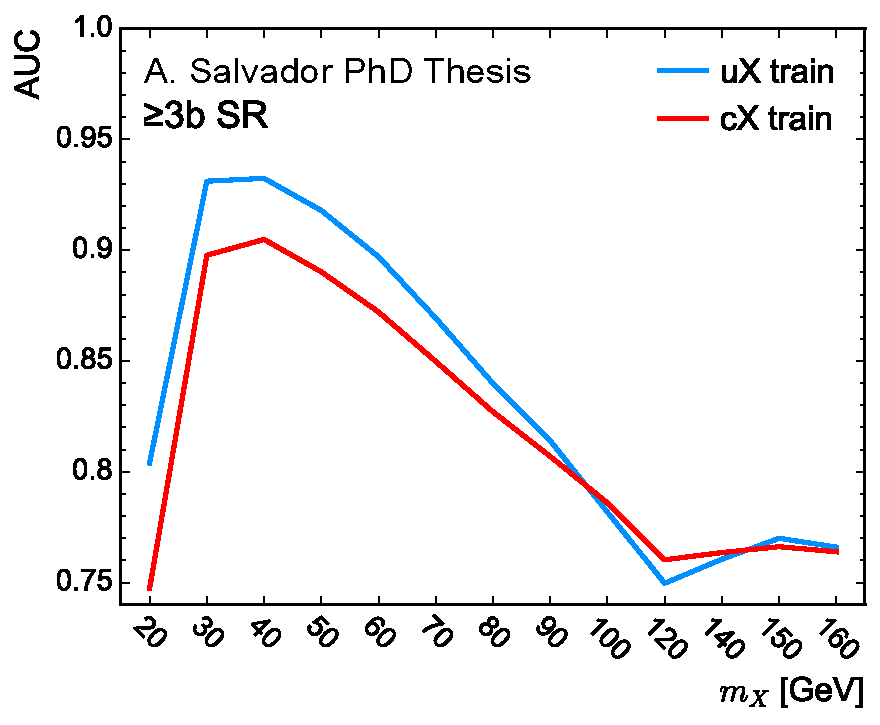
\includegraphics[width = 0.55\textwidth]{TQX/NNcomparison/AUC.pdf}

    \caption{Comparison of the performance, measured as the area of the ROC curve as a function of the mass of the scalar $X$ for the $\ge$3b regions. The NNs are trained using either the $t\to uX$ (blue) or $t\to cX$ (red) samples, and evaluated accordingly.
    }
    \label{tqX:NNAUC}
\end{figure}

\clearpage